% =====================================================================
%  RELATÓRIO TÉCNICO DE CICLO DE PROJETO
%  Tópicos em Sistemas Computacionais I (IoT/AIoT) · UFPI · 2026.2
%
%  COMO USAR
%  1. Abra config/dados-da-equipe.tex e preencha. É o único arquivo de
%     configuração que vocês precisam tocar.
%  2. Escreva nos arquivos da pasta conteudo/, na ordem em que aparecem
%     abaixo. Cada um começa com uma caixa cinza explicando o que vai ali.
%  3. Preencha os apêndices A e B com o mapa de barramento (Aula 06) e o
%     orçamento de energia (Aula 08) que a equipe já entregou. Na AP2,
%     os apêndices E e F (checklist e campanha) aparecem sozinhos.
%  4. Antes de entregar, comente a linha \def\MOSTRARNOTAS{} em
%     config/dados-da-equipe.tex para sumir com as caixas de instrução.
%  5. Compile duas vezes, rode o BibTeX e compile mais duas.
%     No Overleaf: basta apertar Recompile (ele faz isso sozinho).
% =====================================================================

\documentclass[
  12pt,
  oneside,
  a4paper,
  sumario=tradicional,
  english,
  brazil
]{abntex2}

% =====================================================================
%  config/pacotes.tex
%  Pacotes e configuracao de aparencia. Voce nao precisa mexer aqui.
% =====================================================================

% --- Codificacao e fontes ---------------------------------------------
\usepackage[T1]{fontenc}
\usepackage[utf8]{inputenc}
\usepackage{lmodern}
\usepackage{microtype}
\usepackage{csquotes}

% --- Graficos, cores e caixas -----------------------------------------
\usepackage{graphicx}
\usepackage{xcolor}
\usepackage{float}
\usepackage[most]{tcolorbox}

% --- Tabelas ----------------------------------------------------------
\usepackage{booktabs}
\usepackage{array}
\usepackage{tabularx}
\usepackage{longtable}
\usepackage{multirow}
\usepackage{makecell}
\usepackage{pdflscape}

% --- Listas, unidades, matematica -------------------------------------
\usepackage{enumitem}
\usepackage{amsmath}
\usepackage{amssymb}
\usepackage{siunitx}
\sisetup{
  output-decimal-marker = {,},
  group-separator       = {.},
  group-minimum-digits  = 4,
  per-mode              = symbol,
  detect-weight         = true,
}
\DeclareSIUnit{\mAh}{mA\cdot h}
\DeclareSIUnit{\Wh}{W\cdot h}
\DeclareSIUnit{\HSP}{HSP}
\DeclareSIUnit{\baud}{Bd}

% --- Codigo-fonte -----------------------------------------------------
\usepackage{listings}
\definecolor{corComentario}{HTML}{4F7942}
\definecolor{corPalavra}{HTML}{0B3D91}
\definecolor{corTexto}{HTML}{8B1A1A}
\definecolor{corFundo}{HTML}{F7F7F7}
\definecolor{corRegua}{HTML}{BFBFBF}
\definecolor{corDestaque}{HTML}{0B3D91}

\lstset{
  basicstyle        = \ttfamily\footnotesize,
  keywordstyle      = \color{corPalavra}\bfseries,
  commentstyle      = \color{corComentario}\itshape,
  stringstyle       = \color{corTexto},
  numbers           = left,
  numberstyle       = \ttfamily\scriptsize\color{corRegua},
  numbersep         = 8pt,
  backgroundcolor   = \color{corFundo},
  frame             = single,
  rulecolor         = \color{corRegua},
  breaklines        = true,
  breakatwhitespace = true,
  showstringspaces  = false,
  tabsize           = 2,
  captionpos        = b,
  extendedchars     = true,
  inputencoding     = utf8,
  literate =
    {á}{{\'a}}1 {é}{{\'e}}1 {í}{{\'i}}1 {ó}{{\'o}}1 {ú}{{\'u}}1
    {Á}{{\'A}}1 {É}{{\'E}}1 {Í}{{\'I}}1 {Ó}{{\'O}}1 {Ú}{{\'U}}1
    {à}{{\`a}}1 {À}{{\`A}}1
    {â}{{\^a}}1 {ê}{{\^e}}1 {ô}{{\^o}}1
    {Â}{{\^A}}1 {Ê}{{\^E}}1 {Ô}{{\^O}}1
    {ã}{{\~a}}1 {õ}{{\~o}}1 {Ã}{{\~A}}1 {Õ}{{\~O}}1
    {ç}{{\c c}}1 {Ç}{{\c C}}1
    {°}{{\textdegree}}1 {º}{{\textordmasculine}}1 {ª}{{\textordfeminine}}1
    {Ω}{{\ensuremath{\Omega}}}1 {µ}{{\ensuremath{\mu}}}1
}

% Linguagem para o firmware do ESP32 (C/C++ estilo Arduino)
\lstdefinestyle{arduino}{
  language  = C++,
  morekeywords = {setup, loop, pinMode, digitalWrite, digitalRead,
                  analogRead, analogWrite, delay, millis, micros,
                  Serial, Wire, SPI, uint8_t, uint16_t, uint32_t,
                  int8_t, int16_t, int32_t, esp_deep_sleep_start,
                  esp_sleep_enable_timer_wakeup, RTC_DATA_ATTR,
                  HIGH, LOW, INPUT, OUTPUT, INPUT_PULLUP, true, false},
}
\lstdefinestyle{terminal}{
  language     = bash,
  numbers      = none,
  basicstyle   = \ttfamily\footnotesize,
  keywordstyle = \color{corPalavra},
}

% --- Referencias cruzadas e links -------------------------------------
\usepackage[brazilian,hyperpageref]{backref}
\usepackage[alf]{abntex2cite}

\renewcommand{\backrefpagesname}{Citado na(s) pagina(s):~}
\renewcommand{\backref}{}
\renewcommand*{\backrefalt}[4]{%
  \ifcase #1 %
    Nenhuma citacao no texto.%
  \or
    Citado na pagina #2.%
  \else
    Citado #1 vezes nas paginas #2.%
  \fi}

% Dados da equipe Estiagem - revisar antes da entrega.
\def\CICLO{2}
% \def\MOSTRARNOTAS{} % DESLIGADO: remove anotacoes do modelo
\newcommand{\tituloProjeto}{Higrolar}
\newcommand{\subtituloProjeto}{Monitoramento conectado de temperatura e umidade relativa do ar: telemetria MQTT e campanha residencial}
\newcommand{\nomeEquipe}{Estiagem (eq04)}
\newcommand{\repositorioEquipe}{Repositório de entrega: URL não informada nos arquivos recebidos}
% Papeis AP2: A CONFIRMAR coletivamente; devem rotacionar em relacao a AP1.
\newcommand{\listaIntegrantes}{%
  \integrante{Raimundo Nonato da Silva Sá Sobrinho}{20249021765}{papel AP2 a confirmar}
  \integrante{Thales Rodrigues Martins}{20229048430}{papel AP2 a confirmar}
  \integrante{Lemuel Cavalcante Lopes}{20209063994}{papel AP2 a confirmar}
  \integrante{Zacarias do Nascimento Seriano Junnior}{20189037130}{papel AP2 a confirmar}
  \integrante{Francisco de Assis Machado dos Santos}{20199017187}{papel AP2 a confirmar}
  \integrante{Maria do Rosário de Fátima Martins Ferreira}{20229006190}{papel AP2 a confirmar}
}
\newcommand{\instituicaoCurso}{Universidade Federal do Piauí}
\newcommand{\unidadeCurso}{Centro de Ciências da Natureza}
\newcommand{\programaCurso}{Departamento de Computação}
\newcommand{\nomeDisciplina}{Tópicos em Sistemas Computacionais I --- Internet das Coisas e AIoT}
\newcommand{\periodoLetivo}{2026.2}
\newcommand{\docenteDisciplina}{Prof. Atos Apollo Silva Borges}
\newcommand{\localEntrega}{Teresina}
\newcommand{\dataEntrega}{25 de outubro de 2026}
\newcommand{\resumoUsoIA}{IA generativa foi utilizada como apoio à revisão do firmware, aos scripts, à análise dos dados e à redação do relatório; ver Apêndice~\ref{ap:ia}.}

% =====================================================================
%  config/comandos.tex
%  Chaves do ciclo, caixas de apoio e macros do relatório.
%  A equipe não precisa mexer aqui.
% =====================================================================

% ---------------------------------------------------------------------
%  1. CICLO DE PROJETO (AP1, AP2 ou AP3)
% ---------------------------------------------------------------------
\ifdefined\CICLO\else\def\CICLO{1}\fi
\newcounter{ciclo}
\setcounter{ciclo}{\CICLO}

% \seAP{n}{texto}     -> aparece somente no ciclo n
% \aPartirDaAP{n}{t}  -> aparece do ciclo n em diante
\newcommand{\seAP}[2]{\ifnum\value{ciclo}=#1\relax#2\fi}
\newcommand{\aPartirDaAP}[2]{\ifnum\value{ciclo}<#1\relax\else#2\fi}

\newcommand{\nomeciclo}{%
  \ifcase\value{ciclo}\or
    Ciclo de Projeto 1 --- sistema embarcado de sensoriamento e atuação\or
    Ciclo de Projeto 2 --- integração à infraestrutura de comunicação e
      formação do conjunto de dados\or
    Ciclo de Projeto 3 --- projeto integrador de AIoT\fi}

\newcommand{\rotuloAP}{AP\arabic{ciclo}}

\newcommand{\moduloDoCiclo}{%
  \ifcase\value{ciclo}\or Módulo 1\or Módulo 2\or Módulo 3\fi}

% ---------------------------------------------------------------------
%  2. NOTAS AO AUTOR (instruções que somem na versão final)
% ---------------------------------------------------------------------
\newif\ifmostrarnotas
\ifdefined\MOSTRARNOTAS\mostrarnotastrue\else\mostrarnotasfalse\fi

\newtcolorbox{tcbnota}{
  enhanced, breakable,
  colback   = gray!6,
  colframe  = gray!45,
  boxrule   = 0.4pt,
  left      = 6pt, right = 6pt, top = 5pt, bottom = 5pt,
  fontupper = \small\sffamily,
  borderline west = {2pt}{0pt}{gray!55},
  sharp corners,
  before skip = 8pt, after skip = 8pt,
}

\usepackage{comment}
\ifmostrarnotas
  \newenvironment{orientacao}{\begin{tcbnota}\noindent\textbf{Como preencher.}\ }%
                       {\end{tcbnota}}
  \newenvironment{exemploguia}{\begin{tcbnota}\noindent\textbf{Exemplo.}\ }%
                          {\end{tcbnota}}
\else
  \excludecomment{orientacao}
  \excludecomment{exemploguia}
\fi

% ---------------------------------------------------------------------
%  3. DECISÃO DE PROJETO
%     Vale 25% da nota da AP. Uma caixa por decisão que a equipe tomou.
% ---------------------------------------------------------------------
\newcounter{decisao}
\renewcommand{\thedecisao}{DP-\arabic{decisao}}

\newtcolorbox[use counter=decisao]{caixadecisao}[1]{
  enhanced, breakable,
  colback    = corDestaque!4,
  colframe   = corDestaque!70,
  boxrule    = 0.6pt,
  left       = 7pt, right = 7pt, top = 6pt, bottom = 6pt,
  sharp corners,
  fonttitle  = \bfseries\sffamily\small,
  title      = {DP-\thetcbcounter\ --- #1},
  before skip = 10pt, after skip = 10pt,
}

\newenvironment{decisao}[1]{\begin{caixadecisao}{#1}\small}{\end{caixadecisao}}

\newcommand{\campoDecisao}[2]{\par\smallskip\noindent\textbf{#1}\ #2}
\newcommand{\alternativas}[1]{\campoDecisao{Alternativas consideradas.}{#1}}
\newcommand{\criterio}[1]{\campoDecisao{Critério de escolha.}{#1}}
\newcommand{\escolha}[1]{\campoDecisao{Decisão.}{#1}}
\newcommand{\evidencia}[1]{\campoDecisao{Evidência (número e procedência).}{#1}}
\newcommand{\consequencia}[1]{\campoDecisao{Consequência assumida.}{#1}}

% ---------------------------------------------------------------------
%  4. IDENTIFICADORES E VEREDITOS
% ---------------------------------------------------------------------
\newcommand{\RF}[1]{\mbox{\textbf{RF-#1}}}      % requisito funcional
\newcommand{\RNF}[1]{\mbox{\textbf{RNF-#1}}}    % requisito não funcional
\newcommand{\CT}[1]{\mbox{\textbf{CT-#1}}}      % caso de teste
\newcommand{\DP}[1]{\mbox{\textbf{DP-#1}}}      % decisão de projeto

\definecolor{corAprovado}{HTML}{1B6B3A}
\definecolor{corReprovado}{HTML}{9B1C1C}
\definecolor{corParcial}{HTML}{8A6100}
\newcommand{\aprovado}{\textcolor{corAprovado}{\textbf{atende}}}
\newcommand{\reprovado}{\textcolor{corReprovado}{\textbf{não atende}}}
\newcommand{\parcial}{\textcolor{corParcial}{\textbf{atende em parte}}}

% ---------------------------------------------------------------------
%  5. ETIQUETA DA RUBRICA
%     Marca discretamente a que fatia da nota a seção responde.
% ---------------------------------------------------------------------
\newcommand{\rubricaTag}[2]{%
  \par\vspace{-6pt}\noindent
  {\footnotesize\sffamily\color{gray!75}%
   Rubrica da \rotuloAP: #1 --- #2\,\%}%
  \par\vspace{4pt}}

\newcommand{\rubricaFuncionalidade}{\rubricaTag{funcionalidade do protótipo}{30}}
\newcommand{\rubricaJustificativa}{\rubricaTag{justificativa técnica das decisões}{25}}
\newcommand{\rubricaRobustez}{\rubricaTag{robustez, testes e documentação}{25}}
\newcommand{\rubricaComunicacao}{\rubricaTag{comunicação dos resultados}{20}}

% ---------------------------------------------------------------------
%  6. ATALHOS DE TABELA
% ---------------------------------------------------------------------
\newcolumntype{L}[1]{>{\raggedright\arraybackslash}p{#1}}
\newcolumntype{C}[1]{>{\centering\arraybackslash}p{#1}}
\newcolumntype{R}[1]{>{\raggedleft\arraybackslash}p{#1}}
\newcommand{\cabecalholinha}{\rowcolor{gray!12}}
\renewcommand{\arraystretch}{1.25}

% Procedência de um número: folha de dados, bancada ou estimativa.
\newcommand{\estimativa}{\textcolor{corParcial}{\textsc{\small estimativa}}}
\newcommand{\bancada}{\textcolor{corAprovado}{\textsc{\small bancada}}}
\newcommand{\folhadedados}{\textsc{\small folha de dados}}

% ---------------------------------------------------------------------
%  7. MARCAS DA MATRIZ DE DECISÃO (AP2)
%     Três marcas apenas: os critérios não se convertem em pontos.
% ---------------------------------------------------------------------
\newcommand{\serve}{\textcolor{corAprovado}{\textbf{serve}}}
\newcommand{\ressalva}{\textcolor{corParcial}{\textbf{com ressalva}}}
\newcommand{\naoserve}{\textcolor{corReprovado}{\textbf{não serve}}}

% =====================================================================
%  config/estilo.tex
%  Capa, folha de rosto, metadados e aparência geral.
%  A equipe não precisa mexer aqui.
% =====================================================================

% --- Lista de integrantes em três formatos ----------------------------
\newcommand{\integrante}[3]{}

\newcommand{\imprimirIntegrantesCapa}{%
  \begingroup
  \renewcommand{\integrante}[3]{##1\par}%
  \listaIntegrantes
  \endgroup}

\newcommand{\imprimirIntegrantesLinha}{%
  \begingroup
  \renewcommand{\integrante}[3]{##1; }%
  \listaIntegrantes
  \endgroup}

\newcommand{\imprimirTabelaIntegrantes}{%
  \begingroup
  \renewcommand{\integrante}[3]{##1 & ##2 & ##3 \\}%
  \noindent
  \begin{tabular}{@{}L{7.4cm}L{3.0cm}L{4.2cm}@{}}
    \toprule
    \textbf{Integrante} & \textbf{Matrícula} & \textbf{Papel no ciclo} \\
    \midrule
    \listaIntegrantes
    \bottomrule
  \end{tabular}%
  \endgroup}

% --- Metadados do abnTeX2 ---------------------------------------------
\titulo{\tituloProjeto}
\autor{\nomeEquipe}
\local{\localEntrega, Piauí}
\data{\dataEntrega}
\instituicao{\instituicaoCurso\par\unidadeCurso\par\programaCurso}
\tipotrabalho{Relatório técnico}
\orientador[Docente:]{\docenteDisciplina}
\preambulo{%
  Relatório técnico do \nomeciclo, apresentado como instrumento da
  \rotuloAP\ da disciplina \nomeDisciplina, \periodoLetivo,
  do \programaCurso\ da \instituicaoCurso.}

% --- Links e metadados do PDF -----------------------------------------
\definecolor{corLink}{HTML}{0B3D91}
\makeatletter
\hypersetup{
  pdftitle    = {\@title},
  pdfauthor   = {\@author},
  pdfsubject  = {\nomeDisciplina},
  pdfkeywords = {IoT}{AIoT}{ESP32}{sistemas embarcados}{UFPI},
  colorlinks  = true,
  linkcolor   = corLink,
  citecolor   = corLink,
  urlcolor    = corLink,
  filecolor   = corLink,
  bookmarksdepth = 4,
  breaklinks  = true,
}
\makeatother

% --- Espaçamentos e listas --------------------------------------------
\setlrmarginsandblock{3cm}{2cm}{*}
\setulmarginsandblock{3cm}{2cm}{*}
\checkandfixthelayout
\setlength{\parindent}{1.3cm}
\setlength{\parskip}{0.2cm}
\setlist{itemsep=1pt, topsep=4pt, parsep=0pt}
\SingleSpacing

% --- Capa customizada --------------------------------------------------
\renewcommand{\imprimircapa}{%
  \begin{capa}
    \centering
    \IfFileExists{figuras/logo-ufpi.png}{%
      \includegraphics[height=2.3cm]{figuras/logo-ufpi.png}\par\vspace{0.6cm}}{}
    {\sffamily
      {\large\MakeUppercase{\instituicaoCurso}\par}
      {\normalsize\MakeUppercase{\unidadeCurso}\par}
      {\normalsize\MakeUppercase{\programaCurso}\par}}
    \vspace{1.6cm}
    {\sffamily\small\MakeUppercase{Equipe \nomeEquipe}\par}
    \vspace{0.5cm}
    {\normalsize\imprimirIntegrantesCapa}
    \vfill
    {\sffamily\bfseries\LARGE\tituloProjeto\par}
    \vspace{0.4cm}
    {\sffamily\large\itshape\subtituloProjeto\par}
    \vspace{1.2cm}
    \rule{0.55\textwidth}{0.6pt}\par
    \vspace{0.6cm}
    {\sffamily\normalsize Relatório técnico da \rotuloAP\par}
    {\sffamily\small\nomeciclo\par}
    \vspace{0.3cm}
    {\small\nomeDisciplina\par}
    {\small\periodoLetivo\ \textbullet\ \docenteDisciplina\par}
    \vfill
    {\large\localEntrega\par}
    {\large\dataEntrega\par}
    \vspace{0.8cm}
  \end{capa}}


% =====================================================================
\begin{document}

\selectlanguage{brazil}
\frenchspacing

% ---------- ELEMENTOS PRÉ-TEXTUAIS -----------------------------------
\pretextual

\imprimircapa
\imprimirfolhaderosto*

\begin{resumo}
Este relatório documenta a segunda avaliação parcial do projeto Higrolar (equipe Estiagem, eq04), uma plataforma residencial de medição de temperatura e umidade relativa com ESP32, DHT11 e OLED SSD1306. O protótipo foi integrado a uma rede Wi-Fi de 2,4 GHz e ao broker EMQX Cloud por MQTT, com telemetria QoS 1, disponibilidade anunciada por estado retido e Last Will, configuração remota do período e armazenamento por assinante Python em CSV. Uma campanha física, realizada de 23/10/2026 às 14h27min27s até 24/10/2026 às 15h56min54s (UTC-3), produziu 3.096 mensagens, incluindo 3.082 telemetrias; a chave lógica (id, boot\_id, seq) revelou 3.080 medições únicas, duas duplicações e nenhuma lacuna interna nas sequências observadas. Foram registradas três inicializações, um horário de medição nulo antes da sincronização NTP e nenhuma falha de leitura do sensor registrada. A temperatura variou de 26,9 a 36,9~\si{\celsius}, e a umidade relativa, de 34\% a 73\%. Experimentos documentados envolveram queda deliberada de Wi-Fi, reinício do nó, interrupção do gravador, umidificação, refrigeração e operação simultânea de aparelhos. No período de 24/10 das 12h59 às 14h10, com ar-condicionado e umidificador ligados, a média observada foi de 30,14~\si{\celsius} e 59,28\% de umidade, sem inferência causal, pois o ambiente não foi controlado. A solução confirmou o caminho completo de dados até o disco e oferece registros temporais úteis à rotulagem no ciclo 3. Limitações são a resolução do DHT11, a fila volátil, a validação TLS não habilitada no firmware embarcado sem CA e a falta de medição instrumental do consumo do rádio.
\vspace{\onelineskip}
\noindent\textbf{Palavras-chave:} Internet das Coisas; ESP32; MQTT; EMQX Cloud; telemetria; qualidade de dados.
\end{resumo}
\begin{resumo}[Abstract]
\begin{otherlanguage*}{english}
This report presents the second stage of Higrolar, a residential temperature and relative-humidity monitoring system based on ESP32, DHT11 and an SSD1306 display. The device uses Wi-Fi and MQTT over an EMQX Cloud broker, publishing QoS 1 telemetry, retained presence status, Last Will messages and remotely configurable sampling periods. A physical campaign from October 23, 2026 at 14:27:27 to October 24, 2026 at 15:56:54 (UTC-3) recorded 3,096 MQTT messages, including 3,082 telemetry messages and 3,080 logically unique readings identified by (id, boot\_id, seq). Two logical duplicates, no detectable internal sequence gaps, three observed boot identifiers, and one missing acquisition timestamp were found. Recorded temperatures ranged from 26.9 to 36.9 degrees Celsius and relative humidity from 34 to 73 percent. Documented tests covered Wi-Fi disruption, recorder reconnection, reboot, humidification, air conditioning and simultaneous operation. From 12:59 to 14:10 on October 24, both devices were running, while the recorded mean was 30.14 degrees Celsius and 59.28 percent relative humidity; this is an observational association rather than causal evidence. The system delivered sensor data to a persistent CSV dataset. Limitations include sensor resolution, volatile local buffering, missing ESP32 server-certificate verification without a configured CA and lack of instrumented radio-current measurements.
\vspace{\onelineskip}
\noindent\textbf{Keywords:} Internet of Things; ESP32; MQTT; EMQX Cloud; telemetry; data quality.
\end{otherlanguage*}
\end{resumo}


\pdfbookmark[0]{\listfigurename}{lof}
\listoffigures*
\cleardoublepage

\pdfbookmark[0]{\listtablename}{lot}
\listoftables*
\cleardoublepage

\begin{siglas}
\item[AP1/AP2] Primeira/segunda avaliação parcial
\item[BLE] Bluetooth Low Energy
\item[CSV] Comma-Separated Values
\item[DHCP] Dynamic Host Configuration Protocol
\item[GPIO] General-Purpose Input/Output
\item[I\textsuperscript{2}C] Inter-Integrated Circuit
\item[IoT] Internet of Things
\item[LWT] Last Will and Testament
\item[MQTT] Message Queuing Telemetry Transport
\item[NTP] Network Time Protocol
\item[NVS] Non-Volatile Storage
\item[QoS] Quality of Service
\item[TLS] Transport Layer Security
\item[UR] Umidade relativa do ar
\end{siglas}


\pdfbookmark[0]{\contentsname}{toc}
\tableofcontents*
\cleardoublepage

% ---------- ELEMENTOS TEXTUAIS ---------------------------------------
\textual

\chapter{Problema e contexto de uso}
\label{cap:problema}
\rubricaJustificativa
\section{Motivação e continuidade da AP1}
A equipe Estiagem desenvolve o Higrolar para acompanhar as condições térmicas de um ambiente residencial em Teresina (PI), onde episódios de ar seco motivam a observação da umidade relativa. O dispositivo combina ESP32, módulo DHT11 e display OLED (EQUIPE ESTIAGEM, 2026); o primeiro ciclo descreveu a motivação, os requisitos embarcados e a indicação de uso de umidificador. A AP2 toma o mesmo conjunto físico e acrescenta conectividade, registros persistentes e dados utilizáveis em análise longitudinal. A operação do umidificador e do ar-condicionado foi realizada por uma pessoa, não por atuadores elétricos comandados pelo ESP32.

\section{Ambiente operacional e fronteiras}
O nó foi empregado em ambiente residencial com acesso a uma rede Wi-Fi de 2,4~GHz e internet. O primeiro ponto de conectividade é o roteador ou ponto de acesso local; o serviço de mensagens encontra-se no EMQX Cloud, fora da residência. A distância física entre ESP32 e roteador não foi aferida com trena e, por isso, não será declarada como valor medido; o atendimento ao requisito de alcance é demonstrado funcionalmente pela associação Wi-Fi e continuidade da campanha. O computador com Windows 11 executa o assinante Python e grava as mensagens em disco.

\section{Questão do segundo ciclo}
A pergunta investigada na AP2 é: \emph{como tornar auditáveis, recuperáveis e úteis as observações de temperatura e umidade feitas por um nó doméstico, inclusive quando ocorrem interrupções de rede ou reinicializações?} O sucesso exige o caminho completo do sensor ao CSV, critérios verificáveis de qualidade, registro de intervenções ambientais e documentação das decisões de rádio e protocolo.
\section{Escopo do experimento}
A campanha registra mudanças naturais do ambiente e intervenções anunciadas, como ligar o umidificador, ligar o ar-condicionado e operar ambos conjuntamente. As observações não constituem ensaio clínico nem calibração metrológica; o objetivo é caracterizar tendências e eventos rotulados no mesmo ambiente, com limitações de causalidade explicitadas.

\chapter{Requisitos e critérios de aceitação}
\label{cap:requisitos}
\rubricaRobustez
\section{Requisitos funcionais}
\begin{table}[H]\centering\caption{Requisitos funcionais verificáveis na AP2}\label{tab:rf}\scriptsize
\begin{tabular}{@{}L{1.2cm}L{6.1cm}L{7.1cm}@{}}\toprule
\textbf{ID}&\textbf{Comportamento requerido}&\textbf{Critério verificável}\\\midrule
\RF{01}&Ler DHT11 e atualizar exibição local&Leituras a cada 2~s; alterações apresentadas no OLED; teste funcional.\\
\RF{02}&Publicar telemetria por Wi-Fi/MQTT&JSON real recebido no EMQX e MQTTX em QoS~1, em intervalo configurável; \CT{01}.\\
\RF{03}&Expor estado e configuração remota&\texttt{online} retido, LWT \texttt{offline} e comando \texttt{periodo\_s} aplicado; \CT{02}, \CT{04}.\\
\RF{04}&Reconectar após falta de conectividade&Retorno autônomo de \texttt{online} e telemetria após teste de cerca de 2~min sem Wi-Fi; \CT{03}.\\
\RF{05}&Distinguir inicializações do nó&\texttt{boot\_id} diferente após EN e sequência reiniciada sem falsa duplicação; \CT{05}.\\
\RF{06}&Persistir e auditar telemetria&CSV acrescido após recepção; executar \texttt{qualidade.py} e reportar lacunas e duplicações; \CT{06}.\\
\RF{07}&Preservar horário de aquisição&Campo \texttt{ts} numérico após sincronismo e \texttt{null} antes de NTP; \CT{07}.\\
\bottomrule\end{tabular}\fonte{Equipe eq04; critérios baseados na implementação efetiva.}\end{table}
\section{Requisitos não funcionais}
\begin{table}[H]\centering\caption{Requisitos não funcionais e sua verificação}\label{tab:rnf}\scriptsize
\begin{tabular}{@{}L{1.2cm}L{5.1cm}L{4cm}L{4.1cm}@{}}\toprule
\textbf{ID}&\textbf{Requisito}&\textbf{Alvo}&\textbf{Verificação}\\\midrule
\RNF{01}&Unicidade lógica&Chave \texttt{id/boot\_id/seq}&Analisador e \CT{05}\\
\RNF{02}&Conservação local sem internet&Fila em RAM de 120 registros&Inspeção do firmware e \CT{03}\\
\RNF{03}&Entrega confiável ao gravador&QoS 1, sessão persistente e \emph{flush} por mensagem&\CT{06}\\
\RNF{04}&Qualidade quantitativa&Contabilizar saltos internos e calcular a completude sobre as leituras esperadas pela agenda&\texttt{qualidade.py} e \CT{08}\\
\RNF{05}&Segurança da comunicação&MQTT/TLS 8883, credenciais segregadas&Inspeção; ressalva no ESP32\\
\RNF{06}&Autonomia e energia&Orçamento explícito e origem dos valores&Apêndice~\ref{ap:energia}; medição elétrica pendente\\
\bottomrule\end{tabular}\fonte{Equipe eq04.}\end{table}
\section{Restrições e hipóteses}
O DHT11 reporta temperatura/umidade em resolução limitada e não cobre umidades inferiores a aproximadamente 20\% UR, restringindo a detecção do extremo seco. A conectividade depende da rede local e de internet; fila em RAM não resiste a desligamento; a memória NVS preserva apenas o contador de inicializações. A contagem de mensagens esperadas para a \emph{campanha} exige descontar etapas com período de 5~s, intervenções e horas em que a aquisição não ocorreu.
\section{Rastreabilidade}\label{sec:rastreabilidade}
\begin{table}[H]\centering\caption{Rastreabilidade da AP2}\label{tab:rastreabilidade}\footnotesize
\begin{tabular}{@{}L{2cm}L{5.1cm}L{3cm}L{4cm}@{}}\toprule
\textbf{Requisitos}&\textbf{Implementação / evidência}&\textbf{Caso}&\textbf{Situação final}\\\midrule
RF-01, RF-02 & Capítulos~\ref{cap:implementacao} e \ref{cap:conectividade}&CT-01&\aprovado\\
RF-03 & Seção~\ref{sec:topicos}; log de comando&CT-02/04&\aprovado\\
RF-04, RNF-02 & Fila local e logs de Wi-Fi&CT-03&\aprovado\\
RF-05, RNF-01 & NVS e log do \texttt{boot\_id}&CT-05&\aprovado\\
RF-06, RNF-03, RNF-04 & Gravador, CSV, analisador&CT-06/08&\aprovado\, com limite de escopo\\
RF-07 & \texttt{ts:null} no CSV&CT-07&\aprovado\\
RNF-05 & TLS no Python; firmware inseguro se sem CA&CT-09&\parcial\\
RNF-06 & Estimativa de energia da AP1, sem medidor&CT-10&\parcial\\
\bottomrule\end{tabular}\fonte{Equipe eq04.}\end{table}

\chapter{Arquitetura e decisões de projeto}
\label{cap:arquitetura}
\rubricaJustificativa
\section{Arquitetura física e lógica}
A Figura~\ref{fig:arquitetura} explicita os dois fluxos: (i) captação local contínua DHT11~$\rightarrow$~ESP32~$\rightarrow$~OLED; (ii) telemetria ao EMQX via Wi-Fi, consumida pelo MQTTX e pelo \texttt{gravador.py}. Com a rede interrompida, a tarefa do sensor permanece independente da tarefa de rede; mensagens pendentes podem ser enfileiradas localmente.
\begin{figure}[H]\centering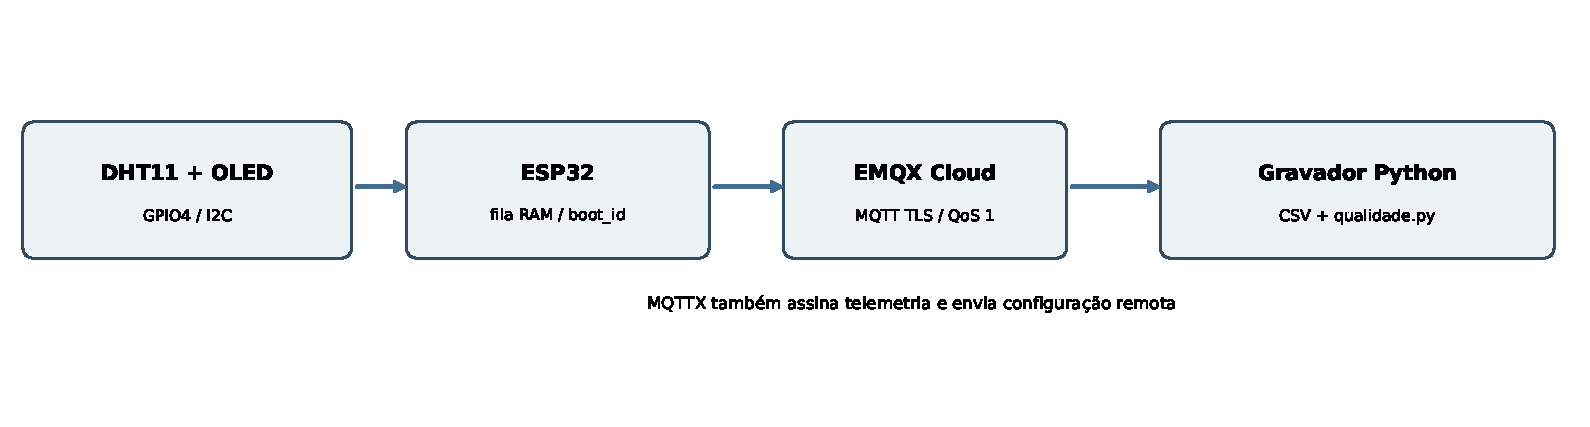
\includegraphics[width=0.94\textwidth]{figuras/arquitetura.pdf}\caption{Arquitetura lógica efetivamente implementada no ciclo 2.}\label{fig:arquitetura}\fonte{Elaborada pela equipe.}\end{figure}
\section{Hardware e barramentos}
O DHT11 utiliza a GPIO4; o OLED SSD1306 de 128$\times$64 usa I\textsuperscript{2}C em SDA/GPIO21 e SCL/GPIO22, endereço \texttt{0x3C}. Ambos usam 3,3~V e terra comum. A leitura do sensor é agendada a cada 2~s; a apresentação visual só é redesenhada quando a indicação muda. As conexões físicas estão consolidadas no Apêndice~\ref{ap:barramento}.
\section{Decisões estruturais}
\begin{decisao}{Separação entre sensoriamento e rede}
\alternativas{Laço de leitura bloqueado por conexão; tarefas cooperativas por \texttt{millis()}.}
\criterio{Continuar lendo o DHT11 a cada 2~s mesmo durante 2~min sem Wi-Fi.}
\escolha{Execução local e reconexão periódica sem laço bloqueante de espera.}
\evidencia{O firmware mantém tarefa de sensor, OLED, Wi-Fi, MQTT e fila separadas.}
\consequencia{A fila de 120 registros limita recuperação; sem alimentação as leituras não publicadas são perdidas.}
\end{decisao}
\begin{decisao}{Identificador por inicialização}
\alternativas{Somente \texttt{seq}; sequência persistente por escrita frequente; \texttt{boot\_id} persistente e \texttt{seq} volátil.}
\criterio{Separar dois registros \texttt{seq=1} em reinícios distintos sem gravar NVS a cada 30~s.}
\escolha{Persistir \texttt{boot\_id} uma vez por inicialização, via \texttt{Preferences}.}
\evidencia{Arquivo final registra \texttt{boot\_id}=120, 121 e 122 e duas duplicatas reais pela chave composta.}
\consequencia{Zerar fisicamente a NVS ou desgaste/falha de gravação pode quebrar a monotonicidade; não representa UUID global.}
\end{decisao}
\begin{decisao}{Persistência no assinante}
\alternativas{Exclusivamente visualizar no MQTTX; CSV por assinante com sessão persistente.}
\criterio{Sustentar uma coleta que atravessa períodos com notebook desconectado, sem descartar eventos e metadados.}
\escolha{Assinante Python com cliente fixo, QoS~1, \texttt{manual\_ack=True}, \texttt{flush()} e \texttt{fsync()} por registro.}
\evidencia{O CSV final contém 3.096 mensagens; o log documenta retorno com backlog após pausa do gravador.}
\consequencia{A latência de gravação e as políticas de retenção do broker são fatores externos; duplicatas continuam possíveis com QoS~1.}
\end{decisao}

\chapter{Implementação do protótipo conectado}
\label{cap:implementacao}
\rubricaFuncionalidade
\section{Materiais e implementação embarcada}\label{sec:bom}
O protótipo utiliza ESP32-D0WD-V3, sensor digital DHT11, visor SSD1306 de 0,96~pol, protoboard e cabos. Foi compilado com o pacote ESP32 da Arduino IDE, biblioteca Adafruit DHT, Adafruit SSD1306/GFX, ArduinoJson 7 e \texttt{arduino-mqtt} de Joel Gaehwiler. A alimentação foi realizada por USB/powerbank de acordo com a etapa experimental; não há acionamento elétrico de climatizador ou umidificador.
\subsection{Registro fotográfico do experimento}
As Fotografias~\ref{fig:foto-arranjo}, \ref{fig:foto-climatizador} e \ref{fig:foto-ar} documentam o arranjo físico utilizado na campanha, incluindo o nó IoT sobre protoboard, o computador empregado na programação e supervisão, o climatizador/umidificador portátil e o ar-condicionado de parede usados nas intervenções manuais. Essas imagens complementam os \emph{prints} de software e ajudam a caracterizar o ambiente experimental real em que a coleta foi executada.
\begin{figure}[H]
\centering
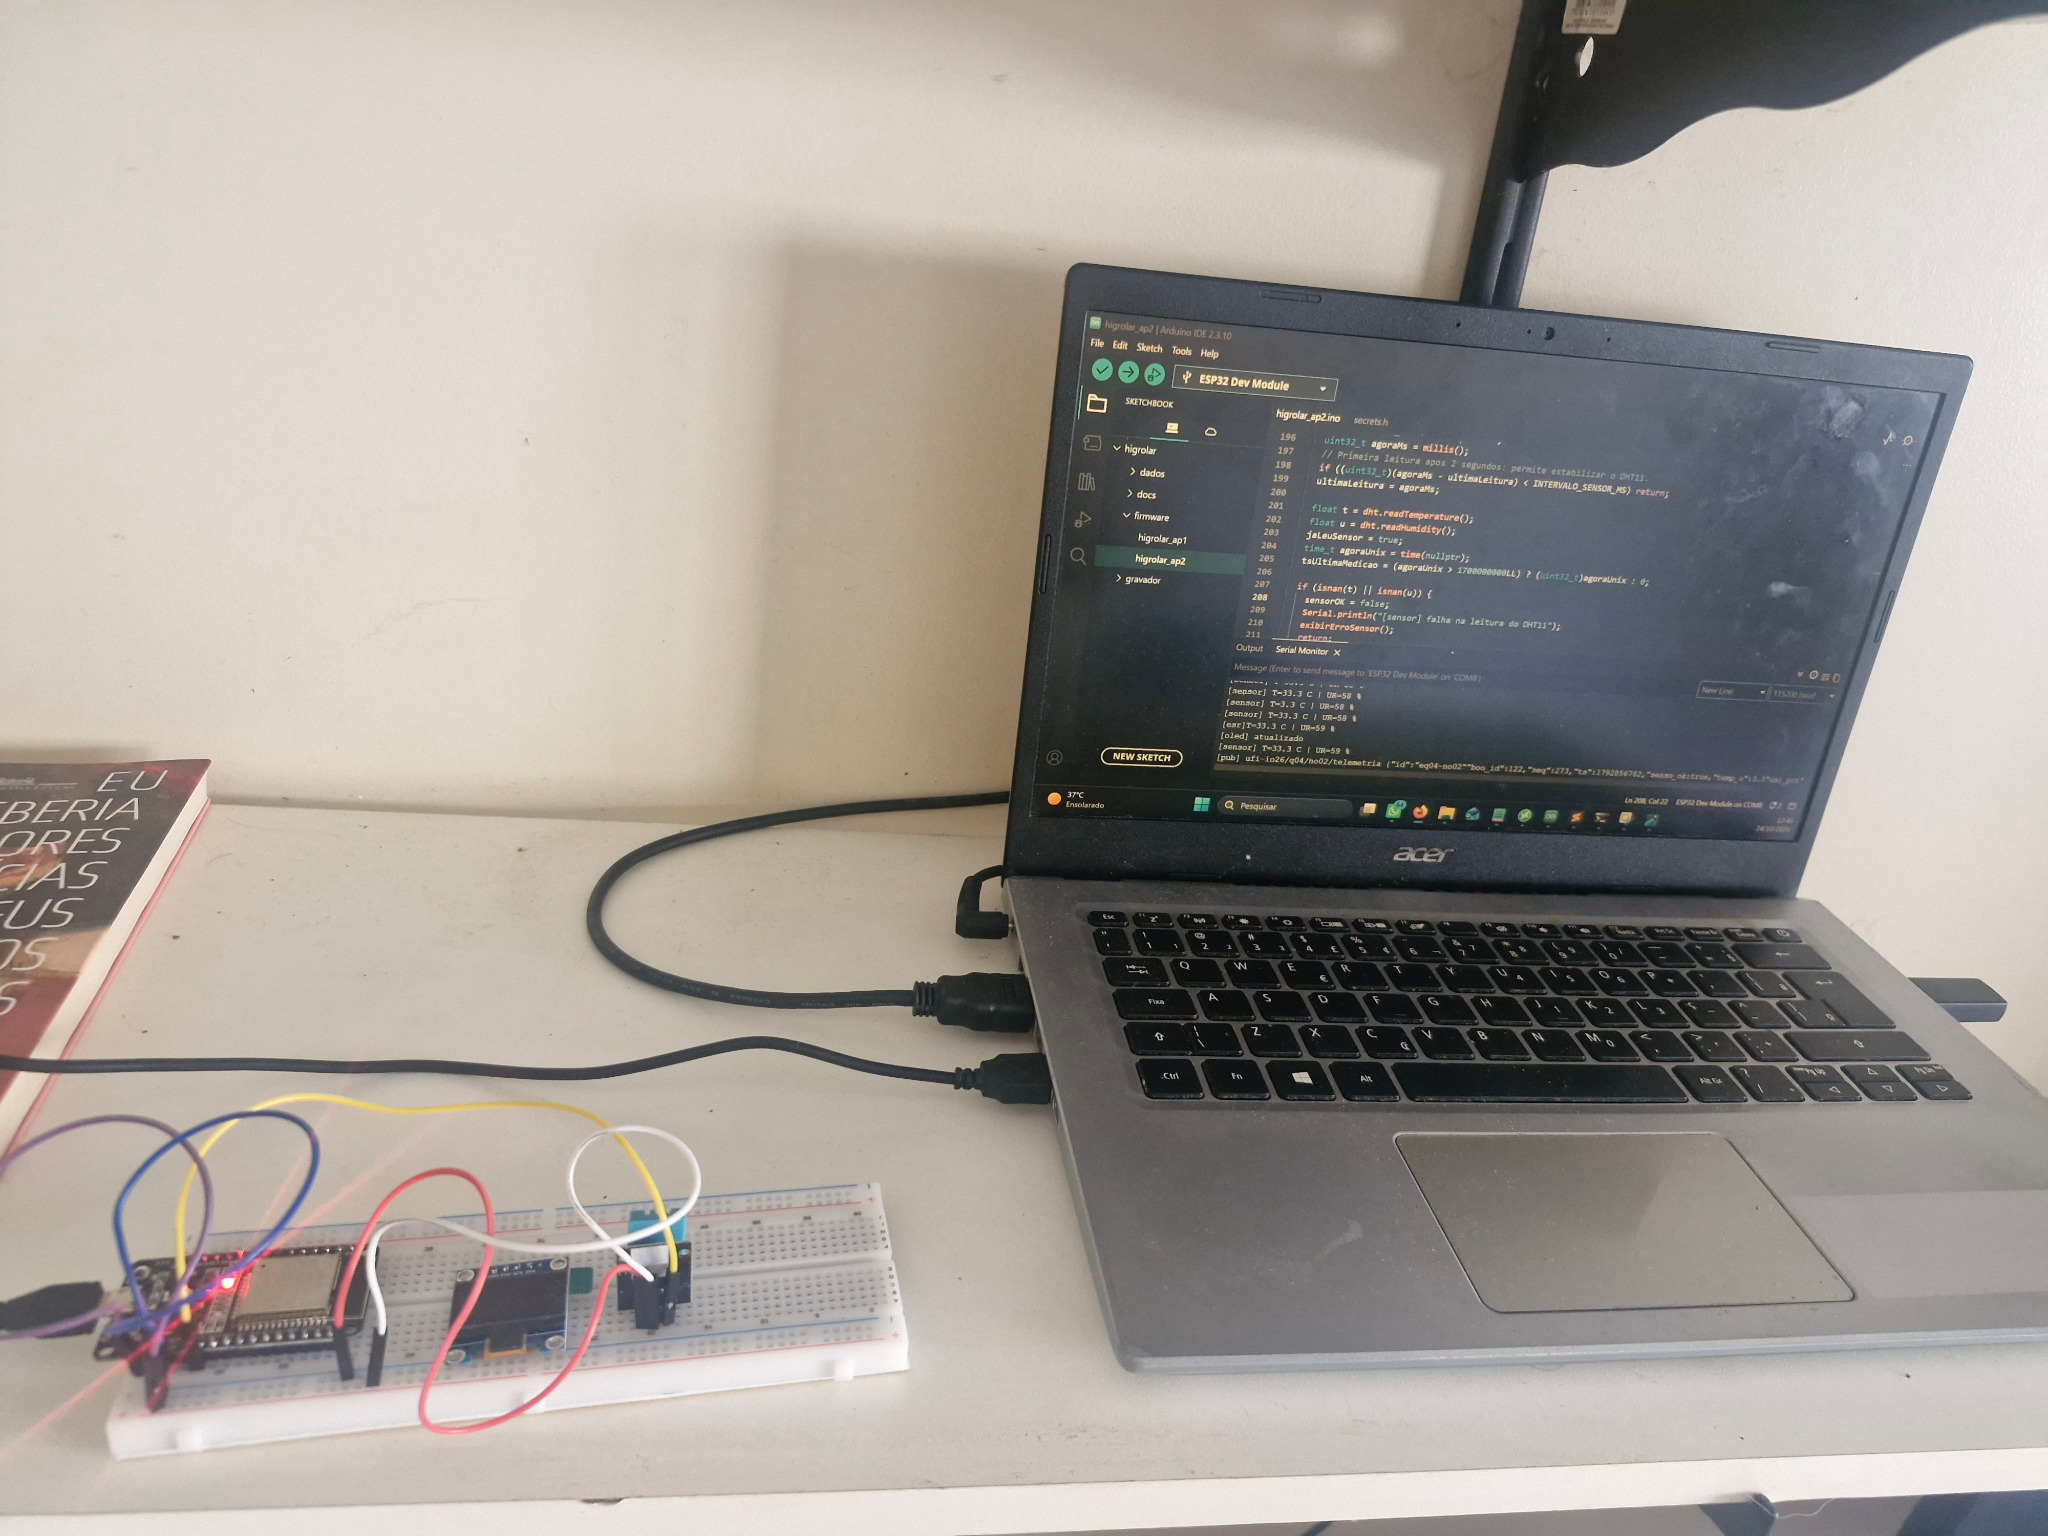
\includegraphics[width=.88\textwidth]{evidencias/fotos/arranjo_experimental.jpg}
\caption{Arranjo experimental de bancada com notebook, ESP32 em protoboard e periféricos usados na campanha.}
\label{fig:foto-arranjo}
\fonte{Fotografia da equipe, 24/10/2026.}
\end{figure}
\begin{figure}[H]
\centering
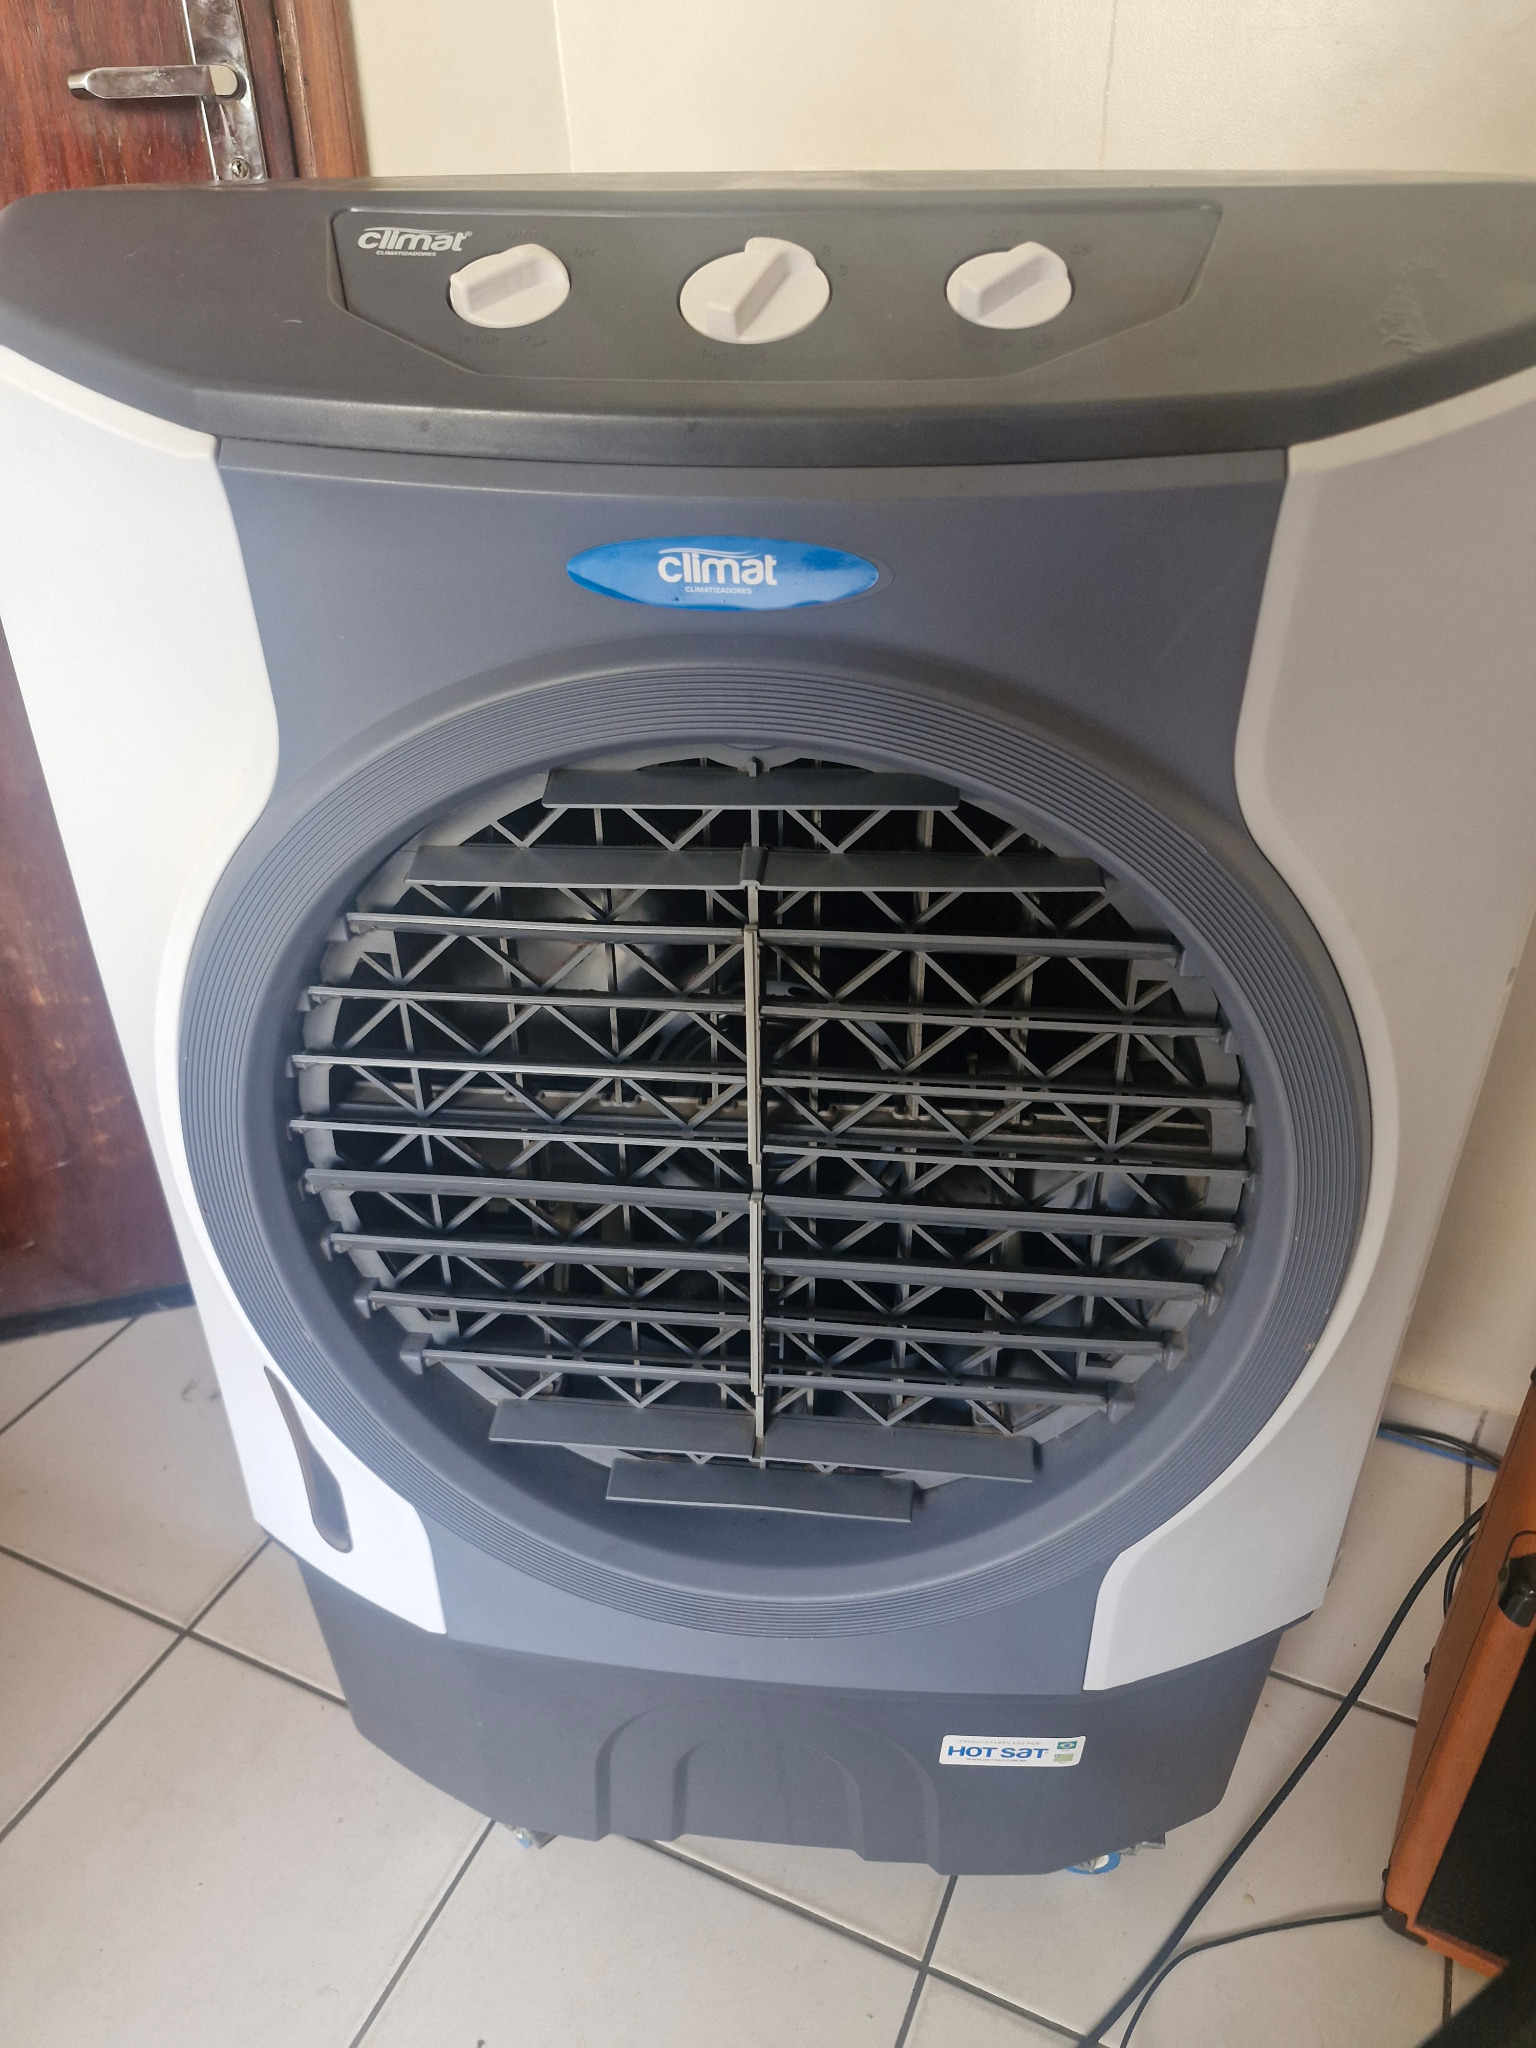
\includegraphics[width=.62\textwidth]{evidencias/fotos/climatizador.jpg}
\caption{Climatizador/umidificador portátil empregado nos ensaios de aumento de umidade e nos testes em operação simultânea.}
\label{fig:foto-climatizador}
\fonte{Fotografia da equipe, 24/10/2026.}
\end{figure}
\begin{figure}[H]
\centering
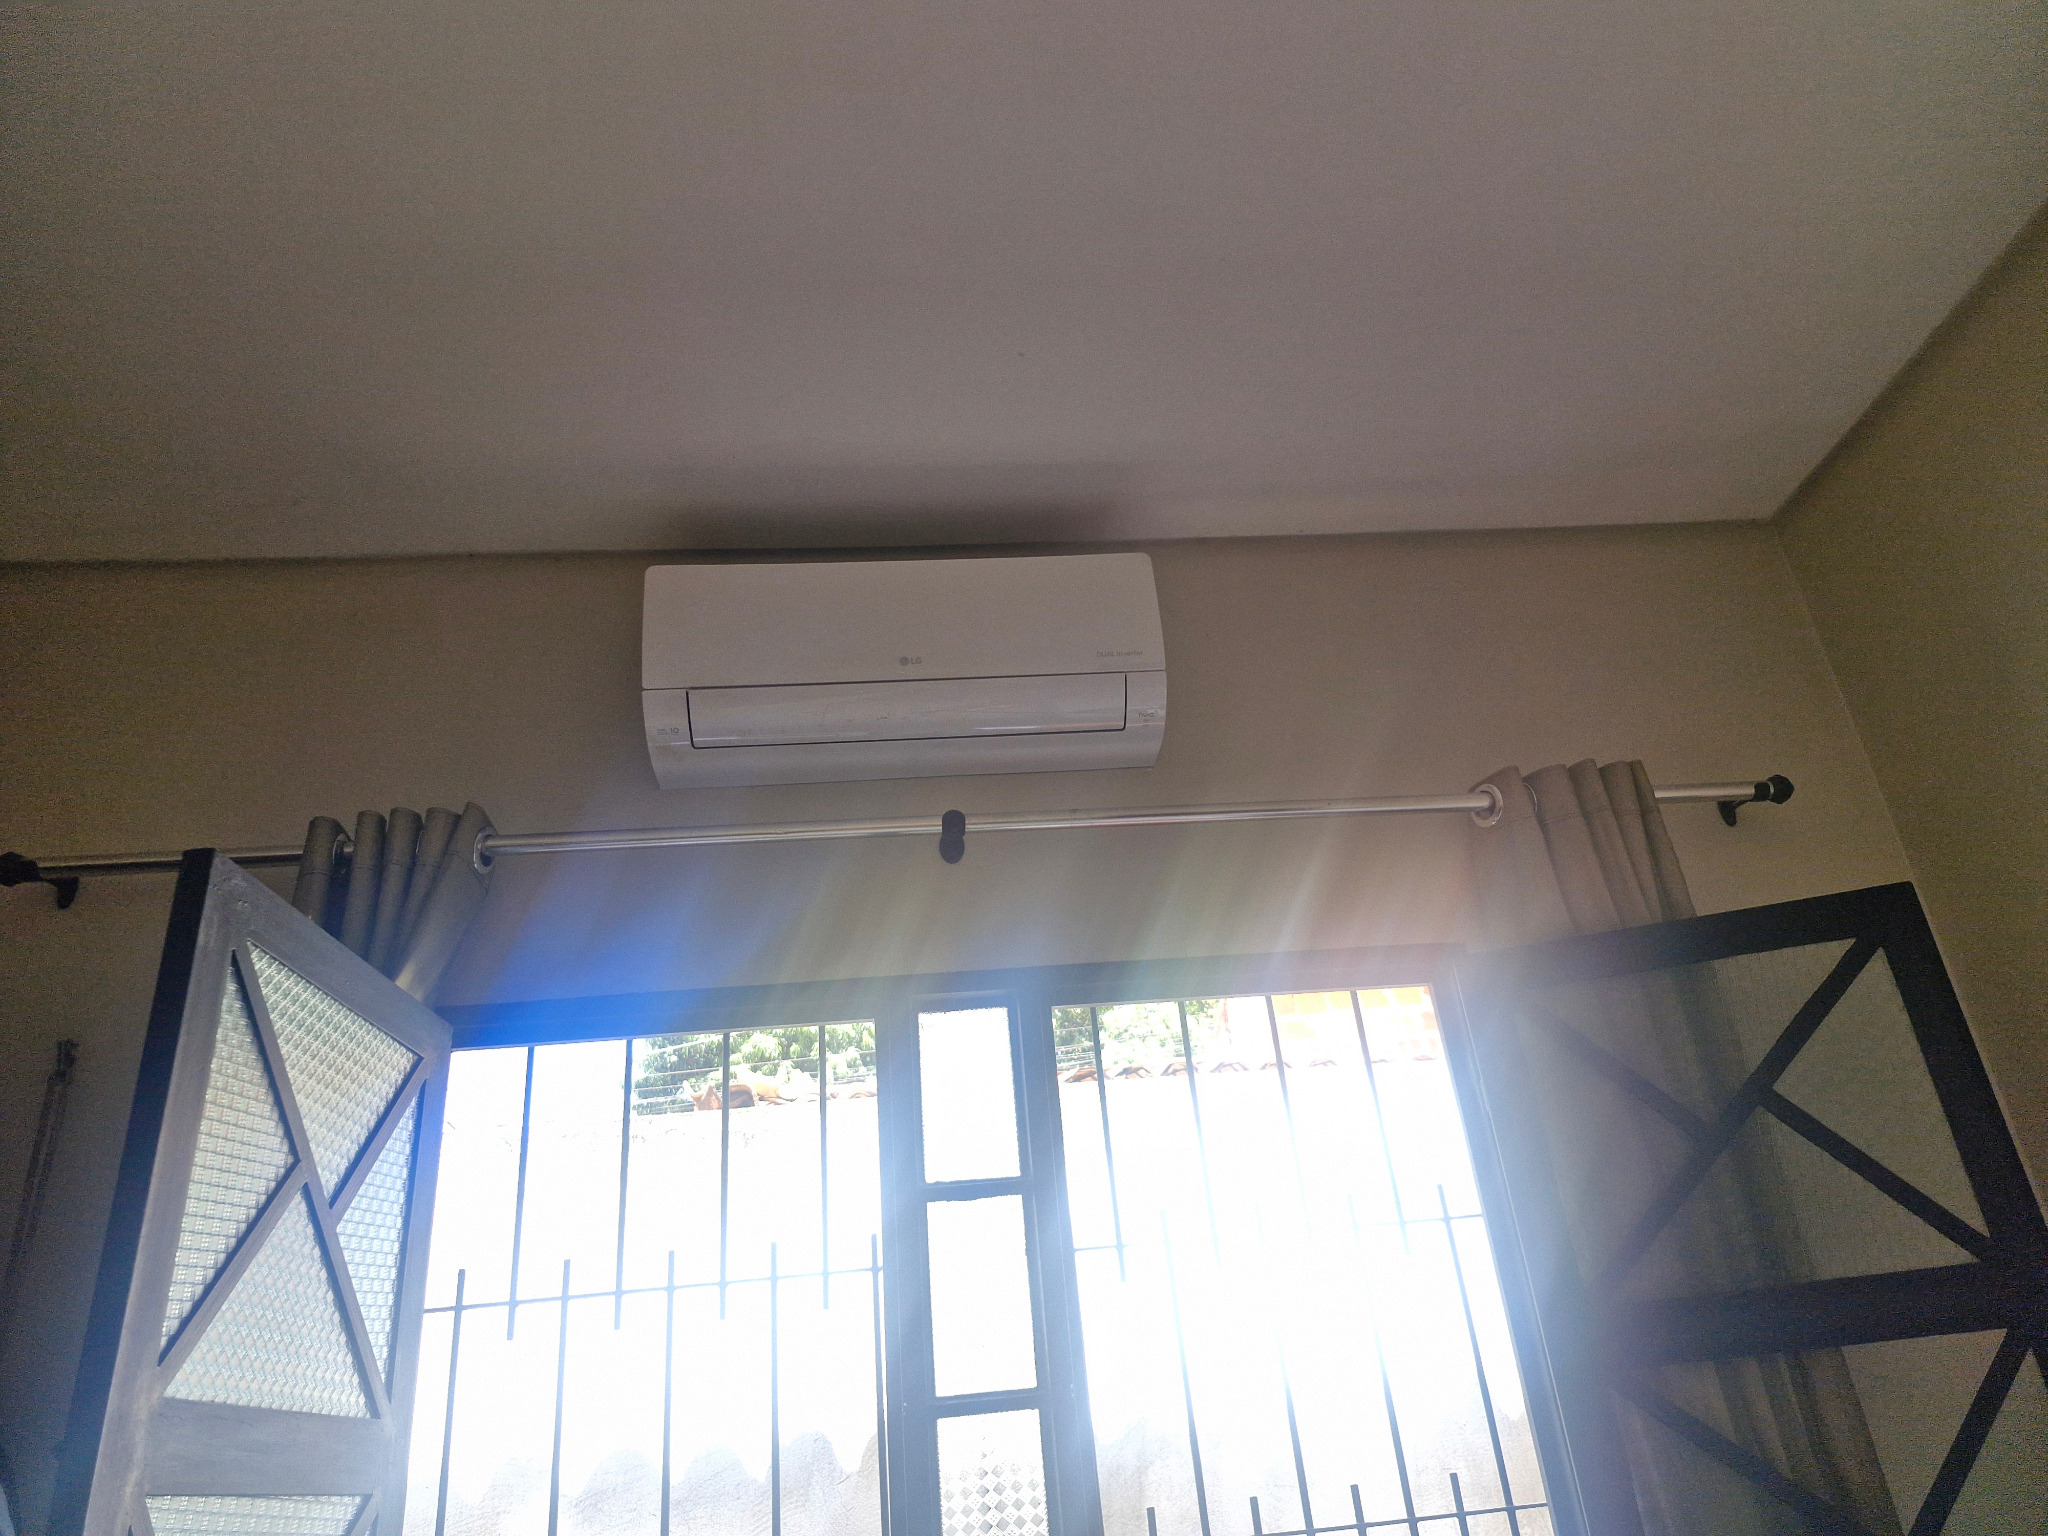
\includegraphics[width=.88\textwidth]{evidencias/fotos/ar_condicionado.jpg}
\caption{Ar-condicionado do ambiente, utilizado nos ensaios de refrigeração isolada e em conjunto com o umidificador.}
\label{fig:foto-ar}
\fonte{Fotografia da equipe, 24/10/2026.}
\end{figure}
\section{Leitura, comunicação e agendamento}\label{sec:firmware}
No \texttt{loop()}, cinco tarefas cooperativas executam leitura do sensor, conexão Wi-Fi, conexão MQTT, agendamento de telemetria e envio da fila, cedendo tempo com \texttt{delay(1)}. Os nomes reais das tarefas estão no código-fonte. O intervalo do sensor é 2~s. O intervalo de publicação inicia em 5~s e é configurado pelo tópico MQTT para 30~s na campanha. A serialização JSON acontece ao descarregar um item da fila; a captura da leitura e sua numeração ocorrem antes, inclusive sem rede.
\begin{lstlisting}[style=arduino,caption={Laço cooperativo do firmware de campanha},label={lst:laco}]
void loop() {
  tarefaSensor();
  tarefaWiFi();
  tarefaMQTT();
  tarefaAgendarTelemetria();
  tarefaEnviarFila();
  delay(1);
}
\end{lstlisting}
O ESP32 gera um contador de inicializações \texttt{boot\_id} salvo pela biblioteca \texttt{Preferences} na NVS. Cada amostra é identificada por \texttt{(id,boot\_id,seq)}; a variável \texttt{seq} reinicia a cada partida, mas o \texttt{boot\_id} muda. A fila circular tem capacidade máxima de 120 registros; quando lotada, o firmware descarta o mais antigo e incrementa a contagem de descartes. A publicação utiliza QoS 1; o retorno de sucesso do método de envio não equivale, por si só, a uma garantia de durabilidade ponta a ponta no CSV.
\section{Estados de conectividade}
A associação Wi-Fi é tentada no início e novamente depois de aproximadamente 15~s sem conexão. MQTT é retentado após 5~s; o assinante de configuração altera \texttt{periodo\_s} entre 2 e 3.600~s. O MQTT usa \emph{keepalive} de 30~s, publicação \texttt{online} retida e testamento \texttt{offline}. O relógio é inicializado por NTP; até haver horário válido o campo \texttt{ts} recebe \texttt{null}.
\section{Gravador, auditoria e rastreabilidade do código}
O \texttt{gravador.py} usa Paho-MQTT 2.x, MQTT 3.1.1 com TLS na porta 8883, sessão persistente e confirmação manual após escrita em CSV. Um certificado confiável é obtido do repositório de autoridades do Windows/sistema por \texttt{ssl.create\_default\_context}; há usuários distintos no EMQX para nó, visualização e gravador. O arquivo resultante preserva horário de recepção, tópico, \texttt{payload}, QoS, flag DUP e campos \texttt{id}, \texttt{boot\_id} e \texttt{seq}. A aplicação de qualidade calcula duplicações por chave composta e intervalos lacunosos por inicialização.
\par\noindent\textbf{Rastreabilidade Git:} o repositório organiza as fontes em \texttt{docs/}; \texttt{firmware/}, em que \texttt{higrolar\_ap2/} é a versão da campanha, com o modelo \texttt{secrets.example.h}; \texttt{gravador/}, com \texttt{gravador.py} e \texttt{qualidade.py}; e \texttt{dados/} (CSV bruto, \texttt{limpar.py} e o CSV limpo derivado dele). O CSV bruto da campanha entrou no \emph{commit} \texttt{e722db7} e não foi alterado depois.
\par\noindent Repositório: \url{\repositorioEquipe}\\
\emph{Commit} correspondente a esta entrega: o marcado pela \emph{tag} \texttt{ap2-final}.

\section{Gestão do broker EMQX e segregação de identidade}
A adaptação ao laboratório trocou o host HiveMQ de demonstração por uma instância EMQX Cloud, mantendo MQTT 3.1.1, QoS~1 e os três tópicos da equipe. As credenciais de autenticação são distintas: \texttt{higrolar-esp32} publica telemetria/status e assina configuração; \texttt{higrolar-monitor} assina a árvore e publica comandos de configuração; \texttt{higrolar-gravador} assina a árvore para persistir dados. Os \emph{client IDs} também são distintos. As permissões vistas no painel são documentadas na Seção~\ref{sec:topicos}; como a autorização estava em \emph{blacklist}, tais regras explícitas não garantem negação de operações não correspondentes. O gravador valida TLS no Windows, mas o nó utiliza \texttt{setInsecure()} quando não é informado um certificado CA. O arquivo \texttt{secrets.h} não integra o pacote de entrega.


% Capítulo que só existe a partir da AP2 (conectividade)
\ifnum\value{ciclo}>1\relax
  \chapter{Conectividade e conjunto de dados}\label{cap:conectividade}
\rubricaJustificativa
\section{Tecnologia de comunicação}\label{sec:tecnologia}
O nó físico permaneceu num ambiente residencial de Teresina--PI com ponto de acesso doméstico à Internet por Wi-Fi 2,4~GHz; a distância real entre nó e roteador não foi medida. As mensagens de aproximadamente uma centena de bytes não exigem rádio de alta vazão, mas a aplicação precisa tanto enviar leituras periódicas como receber mudanças de configuração. O período da fase estável foi de 30~s (2.880 leituras/dia em operação contínua), e a coleta atravessou mais de um ciclo diurno/noturno. A decisão de comunicação foi quantitativamente motivada pela infraestrutura já disponível, não por uma avaliação fictícia de sinal RSSI.
\begin{table}[H]\centering\caption{Matriz de decisão de conectividade para a instalação observada}\label{tab:matriz}\scriptsize
\setlength{\tabcolsep}{3pt}
\begin{tabular}{@{}L{2.0cm}L{3.1cm}C{1.35cm}C{1.35cm}C{1.45cm}C{1.45cm}L{3.6cm}@{}}\toprule
\textbf{Critério}&\textbf{O que o projeto exige}&\textbf{Wi-Fi}&\textbf{BLE}&\textbf{LoRa/ LoRaWAN}&\textbf{NB-IoT/ LTE-M}&\textbf{Observação}\\\midrule
Alcance necessário&Mesmo cômodo do roteador doméstico; distância não aferida&\serve&\ressalva&\serve&\serve&BLE alcança poucos metros em ambiente interno e exige um central sempre ligado\\
Energia disponível&USB ou \emph{powerbank} de 10.000~mA\,h (Apêndice~\ref{ap:energia})&\ressalva&\serve&\serve&\ressalva&Na tomada não restringe; no \emph{powerbank}, o Wi-Fi é o maior consumo, não medido\\
Dado por transmissão&95 a 104 bytes de JSON a cada 30~s (2.880 mensagens/dia)&\serve&\serve&\naoserve&\serve&LoRaWAN: o JSON excede os 51 bytes do SF12 (AU915) e 2.880 mensagens/dia não cabem nos 30~s de ar por dia do TTN\\
Latência aceitável&Leitura em até um período (30~s); comando \texttt{config} aplicado na publicação seguinte&\serve&\serve&\ressalva&\serve&Mediana chegada$-$\texttt{ts} de 2,076~s (Tabela~\ref{tab:qualidade}); em LoRaWAN classe A o \emph{downlink} espera um \emph{uplink}\\
Infraestrutura no local&Wi-Fi 2,4~GHz e internet já existentes; nenhum \emph{gateway}, módulo LoRa ou chip celular&\serve&\naoserve&\naoserve&\naoserve&O kit não tem módulo LoRa nem modem celular; BLE precisaria de um \emph{gateway} para a internet\\
\bottomrule\end{tabular}\fonte{Elaborada pela equipe; as marcas de BLE, LoRaWAN e NB-IoT são avaliações técnicas, sem ensaio físico.}\end{table}
\begin{decisao}{Wi-Fi e MQTT 3.1.1 com EMQX Cloud}
\alternativas{Wi-Fi com MQTT, BLE mediante gateway, LoRaWAN mediante gateway e rede celular com modem.}
\criterio{Reaproveitar hardware e rede já presentes, permitir assinantes independentes e duas direções de mensagem sem gateway adicional.}
\escolha{Wi-Fi 2,4~GHz do ESP32; MQTT QoS 1 sobre o EMQX Cloud na porta 8883/TLS.}
\evidencia{3.082 telemetrias chegaram ao arquivo de disco, incluindo reconexões e comandos remotos; regularidade de 30~s no segmento de operação estável.}
\consequencia{Dependência de Wi-Fi e Internet; consumo do rádio não instrumentado; necessidade de gestão das credenciais e certificados. A escolha deixaria de valer se o nó fosse instalado fora do alcance do roteador (por exemplo, numa área externa da casa) ou tivesse de operar semanas só com bateria: nesse caso a leitura agregada, em formato binário de poucos bytes e com período de minutos, caberia em LoRaWAN, e um \emph{gateway} passaria a fazer parte do projeto.}
\end{decisao}
\section{Caminho do dado: do sensor ao CSV}\label{sec:caminho-dado}
O DHT11 é consultado a cada 2~s. A tarefa de telemetria incorpora a última medição em uma fila RAM de 120 entradas, atribuindo a cada registro a chave \texttt{(id, boot\_id, seq)} e um horário NTP quando válido. O cliente MQTT embarcado transmite \texttt{telemetria} para o EMQX. O broker distribui mensagens aos dois assinantes independentes: MQTTX para observação e \texttt{gravador.py} para persistência. O gravador Paho, em Windows, utiliza a sessão de identificador fixo e \texttt{manual\_ack=True}; escreve CSV com \texttt{flush()}, \texttt{fsync()} e posteriormente confirma o recebimento QoS~1. Falha de energia do nó destrói sua fila RAM, mas não apaga o contador persistido na NVS.\par
\begin{figure}[H]\centering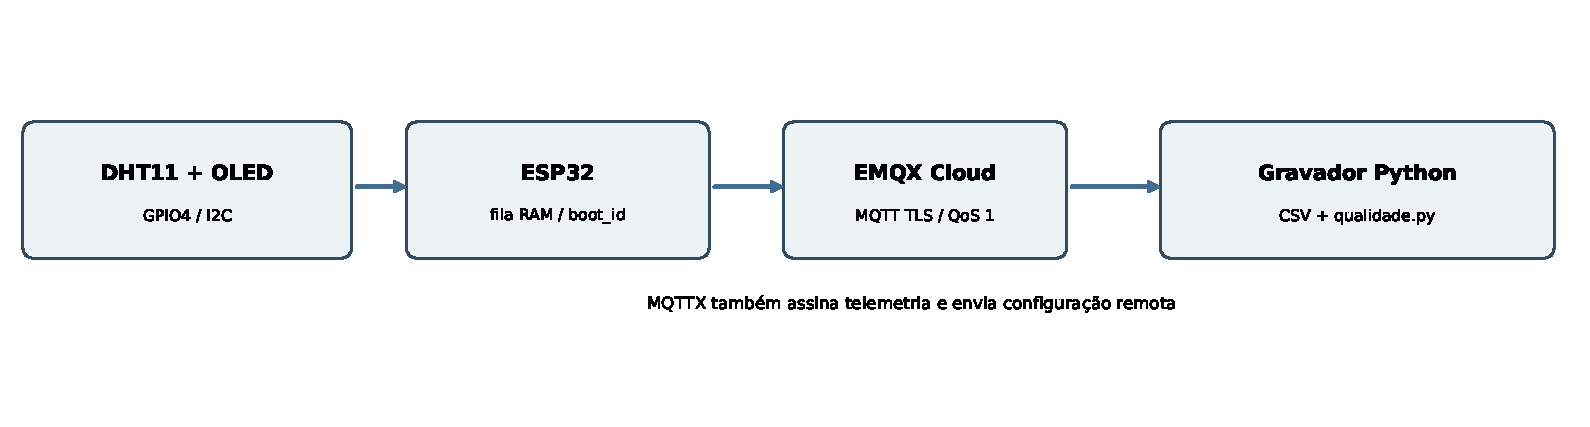
\includegraphics[width=.95\textwidth]{figuras/arquitetura.pdf}\caption{Caminho físico e lógico da aquisição ao arquivo CSV, utilizando EMQX Cloud.}\label{fig:caminho-final}\fonte{Equipe eq04.}\end{figure}
\begin{table}[H]\centering\caption{Onde roda cada peça, e o que acontece se ela parar}\label{tab:pecas}\footnotesize
\begin{tabular}{@{}L{3cm}L{5.3cm}L{5.5cm}@{}}\toprule
Componente&Papel na aplicação&Limite operacional\\\midrule
ESP32/DHT11/OLED&Aquisição, exibição, fila e publicação&Sem alimentação, não mede; fila é volátil\\
Wi-Fi local e Internet&Transporta pacotes MQTT/TLS ao broker&Leituras vão para a fila de 120 posições, que cobre 60~min a 30~s; na queda de 23/10 ela segurou 8 leituras\\
EMQX Cloud&Autenticação, autorização, roteamento, sessões, estado retido e LWT&Não substitui armazenamento histórico de dados\\
MQTTX&Recebe dados e publica configuração autorizada&Observação visual, não é gravador científico\\
Python/Paho e CSV, no notebook Windows 11 da residência&Grava mensagens com hora de recepção e metadados&Com sessão persistente o broker guarda as mensagens QoS~1 enquanto ele está parado (3 leituras na parada de 23/10, 14h38); o notebook precisa de internet, energia e disco\\\bottomrule\end{tabular}\fonte{Arquitetura efetivamente usada.}\end{table}
\section{Contrato de dados}\label{sec:contrato-dados}
A mensagem usa um contrato JSON explícito. A numeração \texttt{seq} reinicia após EN, enquanto \texttt{boot\_id}, armazenado na NVS com \texttt{Preferences}, identifica a inicialização. Assim duas mensagens com \texttt{seq=1} de inicializações distintas não representam a mesma leitura. O campo \texttt{ts} representa tempo de aquisição, não tempo de chegada ao notebook; pode valer \texttt{null} antes do ajuste de relógio NTP.
\begin{table}[H]\centering\caption{Campos e unidade do contrato publicado}\label{tab:contrato-dados}\footnotesize
\begin{tabular}{@{}L{2.15cm}L{1.55cm}L{1.9cm}L{3cm}L{4.5cm}@{}}\toprule
Campo&Tipo&Unidade&Exemplo real&Semântica\\\midrule
\texttt{id}&texto&---&\texttt{eq04-no02}&Nó de origem\\
\texttt{boot\_id}&inteiro&---&122&Inicialização NVS\\
\texttt{seq}&inteiro&---&25&Sequência da inicialização\\
\texttt{ts}&inteiro/null&Unix s&1792777341&Aquisição, após NTP\\
\texttt{sensor\_ok}&booleano&---&\texttt{true}&Leitura considerada válida\\
\texttt{temp\_c}&numérico/null&\si{\celsius}&36.3&Temperatura\\
\texttt{umid\_pct}&numérico/null&\%&37&Umidade relativa\\\bottomrule\end{tabular}\fonte{Payload real do CSV de 23/10.}\end{table}
\begin{lstlisting}[style=terminal,caption={Telemetria real com identificador de inicialização},label={lst:payload}]
{"id":"eq04-no02","boot_id":122,"seq":25,
 "ts":1792777341,"sensor_ok":true,
 "temp_c":36.3,"umid_pct":37}
\end{lstlisting}
A linha CSV adicional contém \texttt{t\_chegada}, \texttt{chegada} em ISO 8601, \texttt{topico}, \texttt{retido}, \texttt{payload}, \texttt{qos}, \texttt{dup}, \texttt{id}, \texttt{boot\_id} e \texttt{seq}. Os dois últimos são nulos para mensagens de estado ou configuração.\par
Esta é a versão do contrato que rodou na campanha (\texttt{firmware/higrolar\_ap2}). Ela difere do contrato-base da disciplina em dois pontos: a chave \texttt{boot} chama-se \texttt{boot\_id} e guarda um contador de inicializações na NVS, e a chave \texttt{sensor\_ok} foi acrescentada para que uma leitura inválida do DHT11 chegue ao arquivo marcada, com \texttt{temp\_c} e \texttt{umid\_pct} nulos, em vez de sumir. BLE foi descartado na Tabela~\ref{tab:matriz}; o projeto não usa contrato GATT.\par
\section{Contrato de tópicos, usuários e garantias}\label{sec:topicos}
O broker utilizado é \textbf{EMQX Cloud} (instância própria da equipe), em substituição à configuração HiveMQ do material de laboratório. A decisão foi operacional: utilizar um plano e instância que estavam acessíveis no período da atividade; não se afirma que todo plano HiveMQ seja pago, pois ofertas comerciais podem mudar. O endpoint pertence ao domínio \texttt{emqxsl.com}, na porta MQTT/TLS 8883. As telas de autenticação e autorização foram preservadas sem mostrar senhas.
\begin{table}[H]\centering\caption{Contrato de tópicos sob \texttt{ufpi-iot26/eq04/no02/}}\label{tab:topicos}\scriptsize
\setlength{\tabcolsep}{3pt}
\begin{tabular}{@{}L{1.8cm}L{2.3cm}C{0.7cm}C{1.3cm}L{2.4cm}L{5.7cm}@{}}\toprule
\textbf{Sufixo}&\textbf{Direção}&\textbf{QoS}&\textbf{Retido?}&\textbf{Quem assina}&\textbf{Por quê}\\\midrule
\texttt{telemetria}&nó $\to$ \emph{broker}&1&não&gravador e MQTTX&QoS~1 com sessão persistente não perde leitura com o gravador parado; a duplicata é descartada pelo \texttt{seq}. Sem retenção, um painel recém-aberto não mostra leitura velha como atual\\
\texttt{status}&nó $\to$ \emph{broker} (e testamento)&1&sim&gravador e MQTTX&Retido para que quem conecta saiba na hora se o nó está \texttt{online}; o testamento publica \texttt{offline} quando o nó cai sem avisar\\
\texttt{config}&MQTTX $\to$ \emph{broker} $\to$ nó&1&não&o nó&Muda o período sem regravar o firmware (\texttt{periodo\_s}: 30); QoS~1 porque um comando perdido deixaria o nó a 5~s\\
\bottomrule\end{tabular}\fonte{Elaborada pela equipe, a partir do contrato testado na campanha.}\end{table}
\noindent As quatro decisões que transformam um nó que publica num nó que forma um conjunto de dados:
\begin{description}[style=unboxed, leftmargin=0pt, font=\normalfont\bfseries]
  \item[1. Sessão persistente nos dois lados, com \emph{client ID} fixo.]\hfill\\
    O \emph{client ID} do nó é \texttt{ufpi-iot26-eq04-no02}; o do gravador, \texttt{ufpi-iot26-eq04-gravador}. Os dois conectam com \emph{clean session} desligada. Os IDs são distintos para que um cliente não derrube o outro. Quando o gravador parou às 14h38 de 23/10, o \emph{broker} guardou as leituras \texttt{seq} 16 a 18 do boot 122 e as entregou às 14h39min03s, com \texttt{session\_present} na reconexão.
  \item[2. O que o nó faz quando o \emph{broker} está fora de alcance.]\hfill\\
    A leitura é numerada e entra numa fila circular em RAM de 120 posições: 60~min a 30~s, ou 10~min a 5~s. Com a fila cheia, o firmware descarta a mais antiga e conta o descarte. Na queda de Wi-Fi de 23/10 a fila segurou 8 leituras (\texttt{seq} 14 a 21 do boot 121, carimbadas de 14h28min51s a 14h32min16s), entregues às 14h32min28s com o \texttt{ts} original. A fila não sobrevive a falta de energia.
  \item[3. \emph{Keepalive} e testamento.]\hfill\\
    \texttt{KEEPALIVE} de 30~s; pelo MQTT 3.1.1, o \emph{broker} declara o cliente morto depois de 1,5 $\times$ 30 = 45~s sem pacote e publica o testamento \texttt{offline}, retido. Na queda de 23/10, a última leitura entregue em tempo real foi a de 14h28min21s e a seguinte (14h28min51s) já foi para a fila; o \texttt{offline} apareceu às 14h29min16s, entre 25 e 55~s depois da perda, o que é compatível com o limite de 45~s. O laço não bloqueia além de \texttt{delay(1)}, bem abaixo desse limite.
  \item[4. Segurança mínima.]\hfill\\
    MQTT sobre TLS na porta 8883, com uma conta por papel no EMQX (Tabela~\ref{tab:contas}). As credenciais ficam em \texttt{secrets.h}, fora da árvore entregue, e o repositório traz só \texttt{secrets.example.h}. O gravador valida o certificado do servidor; o nó não, como descrito abaixo.
\end{description}
Foram cadastradas três identidades na autenticação MQTT do EMQX, com senhas separadas e \emph{client IDs} distintos. Elas cumprem papéis funcionais (não equivalem a permissões administrativas do painel). O modo de autorização exibido no EMQX é \emph{blacklist}, que permite solicitações não correspondentes a uma regra explícita; embora haja regras \emph{Allow} cadastradas, essa configuração \textbf{não implementa isolamento de acesso por padrão}. A mudança para \emph{whitelist} é recomendação de endurecimento para implantação posterior.
\begin{table}[H]\centering\caption{Contas do EMQX, papéis e permissões configuradas}\label{tab:contas}\scriptsize
\begin{tabular}{@{}L{2.5cm}L{2.55cm}L{4cm}L{5cm}@{}}\toprule
Usuário MQTT&Papel&Permissões exibidas&Uso no projeto\\\midrule
\texttt{higrolar-esp32}&Dispositivo&SUB \texttt{.../config}; PUB \texttt{.../status} e \texttt{.../telemetria}&Publicar leituras/estado; receber período\\
\texttt{higrolar-monitor}&Monitor e controle&SUB \texttt{ufpi-iot26/eq04/\#}; PUB \texttt{.../config}&Visualização MQTTX e comando remoto\\
\texttt{higrolar-gravador}&Coletor&SUB \texttt{ufpi-iot26/eq04/\#}&Paho, sessão persistente, escrita no CSV\\\bottomrule\end{tabular}\fonte{Capturas do painel EMQX na implantação eq04.}\end{table}
\begin{figure}[H]\centering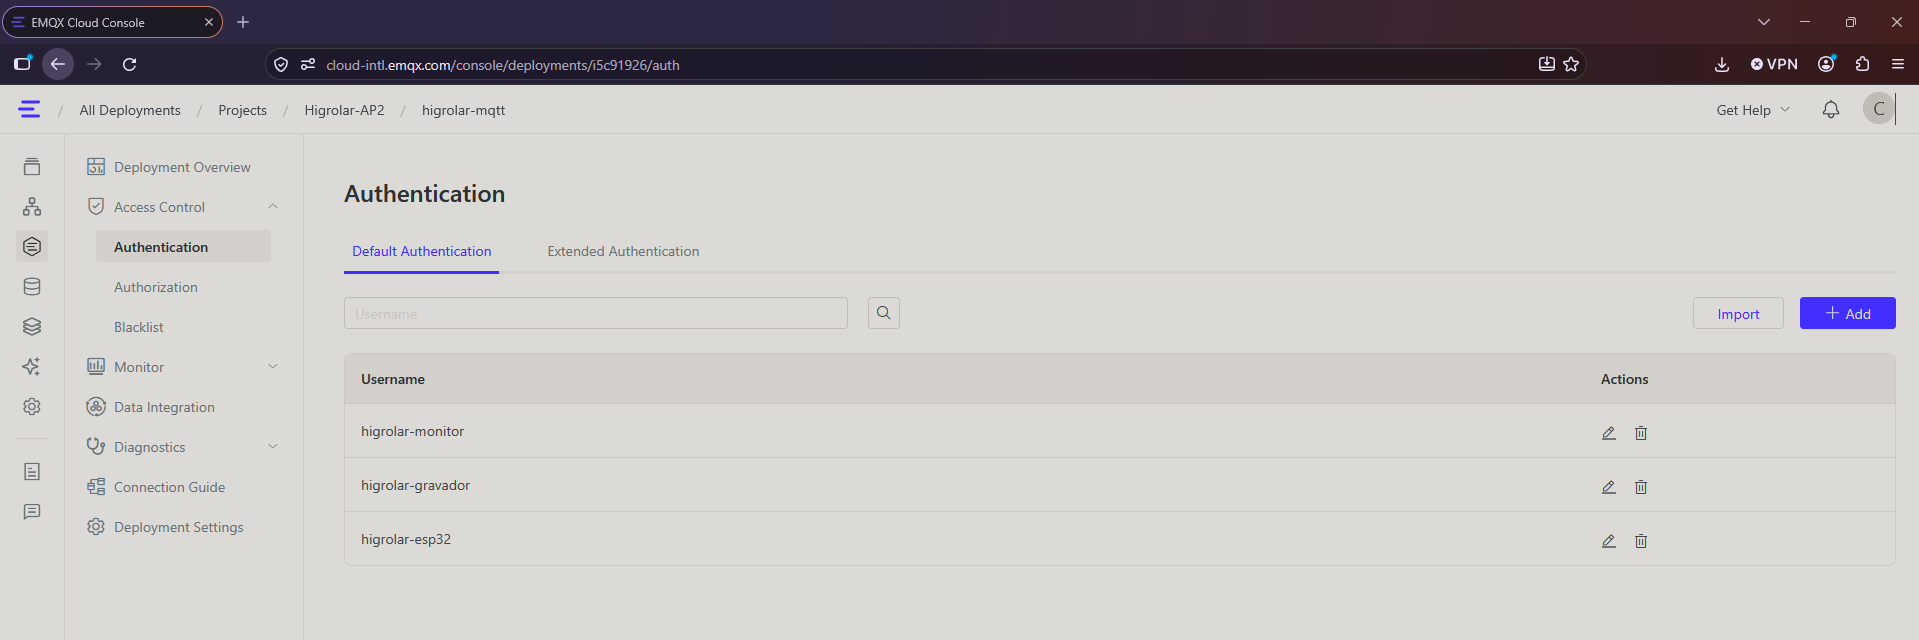
\includegraphics[width=.96\textwidth]{evidencias/prints/emqx_autenticacao.png}\caption{Contas MQTT separadas na autenticação do EMQX Cloud, sem exposição de senhas.}\label{fig:emqx-users}\fonte{Captura da equipe no console EMQX.}\end{figure}
\begin{figure}[H]\centering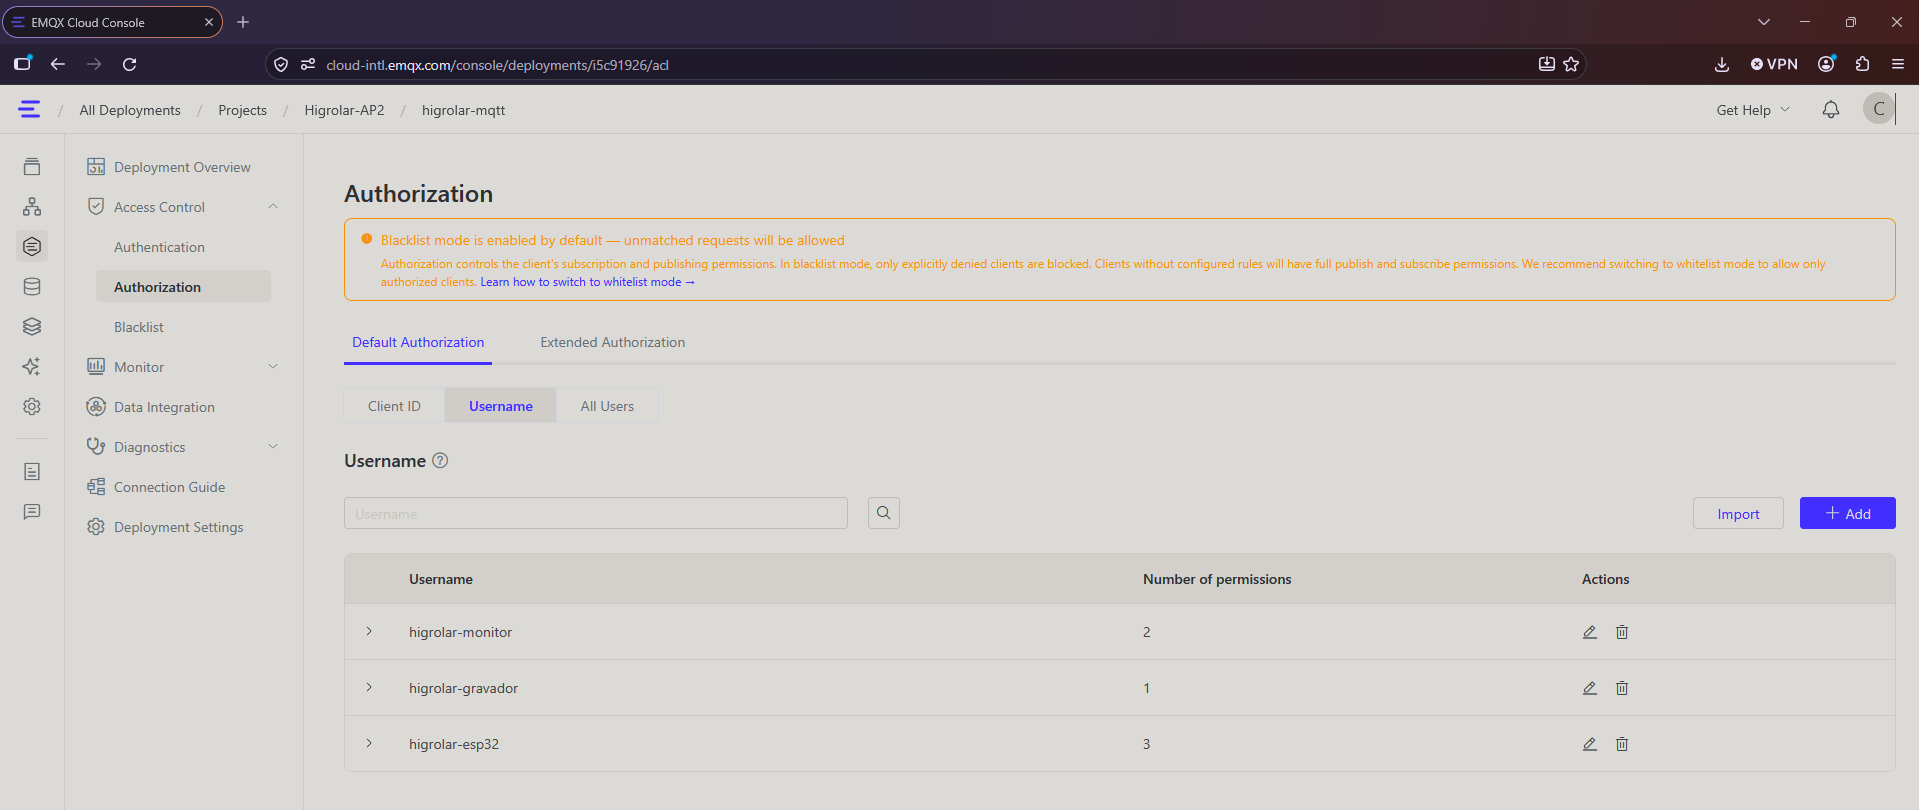
\includegraphics[width=.96\textwidth]{evidencias/prints/emqx_autorizacao.png}\caption{Modo de autorização \emph{blacklist} exibido no EMQX; solicitações sem regra explícita permanecem permitidas.}\label{fig:emqx-mode}\fonte{Captura da equipe no console EMQX.}\end{figure}
\begin{figure}[H]\centering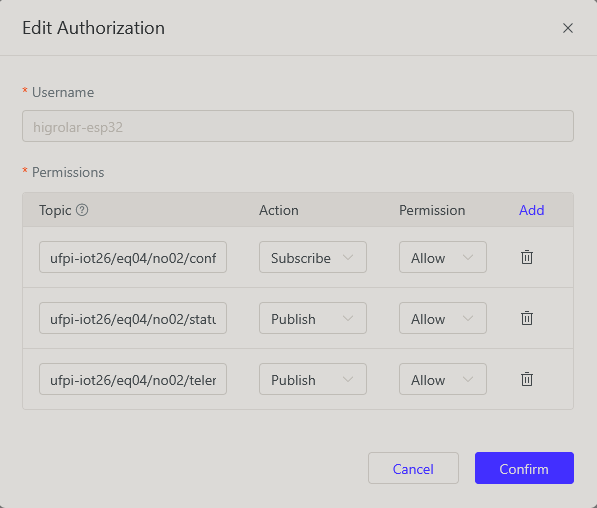
\includegraphics[width=.72\textwidth]{evidencias/prints/emqx_acl_esp32.png}\caption{Regras explícitas de \emph{publish/subscribe} cadastradas para o ESP32.}\label{fig:emqx-esp}\fonte{Captura da equipe.}\end{figure}
\begin{figure}[H]\centering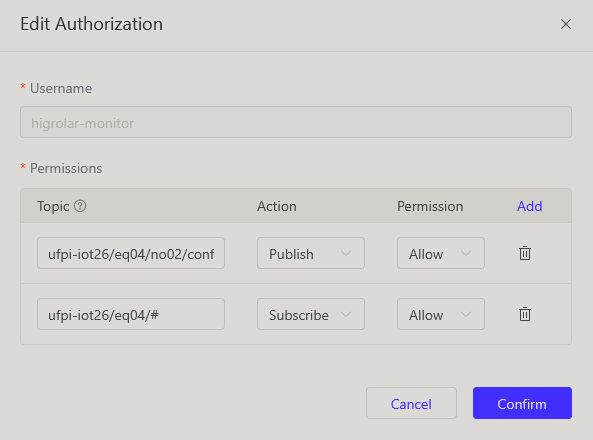
\includegraphics[width=.72\textwidth]{evidencias/prints/emqx_acl_monitor.png}\caption{Regras explícitas do monitor MQTTX: leitura da árvore e escrita em configuração.}\fonte{Captura da equipe.}\end{figure}
No cliente Python, a pilha SSL usa as autoridades certificadoras confiáveis do Windows e verifica a cadeia do servidor. No ESP32, o firmware usado na campanha chama \texttt{setInsecure()} na ausência de \texttt{MQTT\_CA\_PEM}; portanto o enlace é criptografado, mas \textbf{não valida a identidade remota} nessa configuração. Esta distinção é registrada como limitação de segurança, não ocultada pelo sucesso do MQTTX. O LWT \texttt{offline} é retido e publicado pelo broker quando a sessão falha. O QoS~1 permite entrega repetida; o identificador composto resolve duplicações lógicas no conjunto de dados, mas não evita mensagens não geradas ou perdas da fila volátil.\par
\section{Custo da comunicação}\label{sec:custo-radio}
A referência da AP1 era cerca de 75,4~mA de corrente média \emph{estimada}, anterior à ativação de Wi-Fi. A AP2 acrescentou associação, TLS, \emph{keepalive} e publicações de 30 em 30~s. A carga útil ideal de cerca de 100--140 bytes em 2.880 mensagens/dia corresponde a aproximadamente 0,29--0,40 MB/dia \emph{somente de payload}; o tráfego de rede real é maior. \textbf{A equipe não registrou corrente nem tempo do rádio com instrumento}; nenhuma autonomia com rádio é apresentada como medida.
\begin{table}[H]\centering\caption{Procedência do orçamento de energia}\label{tab:custo-radio}\footnotesize
\begin{tabular}{@{}L{4.5cm}L{3.1cm}L{6.5cm}@{}}\toprule
Item&Valor/estado&Origem e restrição\\\midrule
Corrente sem rádio&75,4 mA, estimativa&Orçamento anterior da AP1\\
Corrente rádio e duração de TLS&Não medidas&Requer medidor de corrente / \texttt{millis()}\\
Período de publicação estável&30 s&Comando MQTT e timestamp de aquisição\\
Autonomia real&Não determinada&Não extrapolar sem perfil de corrente\\\bottomrule\end{tabular}\fonte{Código, AP1 e dados da campanha.}\end{table}
O Apêndice~\ref{ap:energia} documenta cenários de sensibilidade; a ausência da medição de rádio permanece um requisito experimental não atendido.\par
\section{Campanha de coleta}\label{sec:campanha}
A campanha foi realizada no protótipo físico em ambiente residencial, com os equipamentos ambientais acionados manualmente e anotados no Apêndice~\ref{ap:campanha}. O intervalo entre a primeira e a última mensagem foi de \textbf{25h29min27s}, de 23/10/2026 às 14h27min27s a 24/10/2026 às 15h56min54s (UTC-3). O início contém os ensaios intencionais de falha e publicações com período de 5~s; a fase estável opera com período MQTT configurado em 30~s. Trata-se de uma janela suficiente para observar a alternância entre períodos diurno/noturno e múltiplas intervenções pontuais, mas não para demonstrar sazonalidade ou generalização.
\begin{table}[H]\centering\caption{Ficha final da campanha}\label{tab:campanha}\footnotesize
\begin{tabular}{@{}L{4.25cm}L{9.75cm}@{}}\toprule
Item&Valor efetivo e base de evidência\\\midrule
Local e nó&Ambiente residencial em Teresina--PI; \texttt{eq04-no02}, ESP32+DHT11+OLED\\
Broker&EMQX Cloud, MQTT 3.1.1, TLS na porta 8883\\
Recorte total&23/10 14h27min27s até 24/10 15h56min54s (UTC-3)\\
Duração do arquivo&25h29min27s\\
Volume MQTT&3.096 mensagens: 3.082 telemetrias, 12 estados e 2 configurações\\
Chaves únicas&3.080 telemetrias distintas por \texttt{(id,boot\_id,seq)}\\
Inicializações&\texttt{boot\_id}=120, 121, 122\\
Período&5~s inicial e 30~s após comando remoto, com interrupções deliberadas\\
Formato/arquivo&CSV bruto UTF-8, \texttt{dados/mensagens.csv}\\
Experimentos&Wi-Fi, reboot, gravador, NTP, umidificador, ar-condicionado, funcionamento conjunto\\
Período de amostragem&30~s; 5~s nos primeiros segundos de cada boot, até chegar o comando \texttt{config}\\
Janela do nó (primeiro e último \texttt{ts})&23/10 14h24min25s a 24/10 15h56min53s: 91.948~s\\
Leituras esperadas (duração $\div$ período)&3.080, somando os trechos da Tabela~\ref{tab:esperadas}\\
Número de nós&1 (\texttt{eq04-no02})\\
Onde rodou o gravador&Notebook com Windows 11 na mesma residência, ligado durante toda a coleta\\
Como a equipe acompanhou a coleta&\texttt{status} e telemetria no MQTTX; \texttt{qualidade.py} rodado durante a coleta (instantâneo de 24/10, 12h08, em \texttt{docs/evidencias/}) e sobre o arquivo final\\
Por que esta duração basta para a AP3&Cobre um ciclo dia--noite completo e oito intervalos de intervenção anotados (Tabela~\ref{tab:eventos}), o bastante para rótulos exploratórios. Não basta para generalizar: cada condição aconteceu uma ou duas vezes, num único cômodo e num único dia\\\bottomrule\end{tabular}\fonte{\texttt{mensagens.csv}, log final de qualidade e diário da equipe.}\end{table}
\noindent\textbf{Leituras esperadas.} A conta sai do tempo em que o nó deveria estar publicando dividido pelo período vigente em cada trecho, e não da contagem de linhas do arquivo. Como o período muda de 5 para 30~s dentro de cada boot, a conta é feita por trecho (Tabela~\ref{tab:esperadas}). Uma conta ingênua, com 30~s na janela inteira, daria $91.948/30 + 1 \approx 3.065$ leituras, menos do que as recebidas, porque ignora os trechos a 5~s. As leituras 1 a 18 do boot 120 não estão no arquivo, que começa na conexão do gravador de 23/10 às 14h27min27s, e ficam fora da conta.
\begin{table}[H]\centering\caption{Leituras esperadas por trecho da campanha}\label{tab:esperadas}\scriptsize
\begin{tabular}{@{}L{2.6cm}L{4.4cm}R{1.5cm}R{1.4cm}R{1.8cm}R{1.8cm}@{}}\toprule
\textbf{Trecho}&\textbf{Início -- fim (\texttt{ts} do nó)}&\textbf{Duração}&\textbf{Período}&\textbf{Esperadas}&\textbf{Únicas recebidas}\\\midrule
boot 120&23/10 14h24min25s -- 14h24min55s&30~s&30~s&2&2\\
boot 121, a 5~s&14h25min14s -- 14h25min51s&37~s&5~s&8&8\\
boot 121, a 30~s&14h25min51s -- 14h33min53s&482~s&30~s&16&16\\
boot 122, a 5~s&14h34min06s\textsuperscript{a} -- 14h34min51s&45~s&5~s&10&10\\
boot 122, a 30~s&14h34min51s -- 24/10 15h56min53s&91.322~s&30~s&3.044&3.044\\\midrule
\textbf{Total}&&&&\textbf{3.080}&\textbf{3.080}\\\bottomrule\end{tabular}\fonte{\texttt{dados/telemetria\_limpa.csv}. Esperadas $= 1 + \lfloor\text{duração}/\text{período}\rfloor$ no primeiro trecho de cada boot e $\lfloor\text{duração}/\text{período}\rfloor$ nos seguintes. \textsuperscript{a}Hora de chegada da leitura com \texttt{ts} nulo.}\end{table}
\section{Qualidade do conjunto de dados}\label{sec:qualidade}
O programa \texttt{qualidade.py} analisou exatamente o mesmo CSV final arquivado no projeto; sua saída completa encontra-se no Apêndice~\ref{ap:campanha}. Identificou 3.082 telemetrias recebidas, 3.080 únicas e duas repetidas pela chave composta; não encontrou saltos entre sequências mínimas e máximas dentro dos três \texttt{boot\_id} observados. Os três boots têm sequências 19--20, 1--24 e 1--3054, respectivamente. A completude de \textbf{100\%} relatada pelo programa é \textbf{interna aos intervalos numerados observados}; não se pode extrapolar automaticamente essa taxa para períodos sem numeração ou mensagens não criadas.
\begin{table}[H]\centering\caption{Indicadores de qualidade do CSV definitivo}\label{tab:qualidade}\footnotesize
\begin{tabular}{@{}L{7cm}R{3.2cm}L{3.1cm}@{}}\toprule
Indicador&Valor&Interpretação\\\midrule
Mensagens no arquivo&3.096&Conjunto final\\
Telemetrias recebidas&3.082&Inclui retransmissões\\
Telemetrias lógicas únicas&3.080&Chave por boot e seq\\
Duplicações lógicas&2&Retidas no CSV bruto\\
Saltos internos de sequência&0&Nos trechos observados\\
Fora de ordem&0&No log analisado\\
Boots observados&3&120, 121, 122\\
\texttt{ts} ausente&1&NTP ainda não válido\\
Falhas de sensor&0&Flag \texttt{sensor\_ok}\\
Atraso mediano (chegada--ts)&2,076~s&Depende dos relógios\\
P95 de chegada--ts&2,521~s&Desconsidera timestamp nulo\\
Máximo de chegada--ts&217,544~s&Inclui backlog intencional\\
Mensagens fora do contrato&0&Todas as 3.082 telemetrias têm as sete chaves da Tabela~\ref{tab:contrato-dados}\\\midrule
Leituras esperadas (conta)&3.080&Tabela~\ref{tab:esperadas}\\
\textbf{Completude}&\textbf{100\,\%}&3.080 únicas / 3.080 esperadas\\\bottomrule\end{tabular}\fonte{\texttt{qualidade.py}; saída literal no Apêndice F.}\end{table}
\noindent\textbf{Denominador da completude.} As leituras esperadas saem da conta da Tabela~\ref{tab:esperadas}, que usa a duração de cada trecho e o período vigente, e não o \texttt{seq}. As 3.080 leituras únicas cobrem as 3.080 esperadas. O resultado vale para a janela em que o nó estava ligado: o que ele não mediu enquanto reiniciava não existe no arquivo. Os dois reinícios duraram menos que um período de 30~s, então nenhuma leitura agendada se perdeu neles (Tabela~\ref{tab:lacunas}).\par
\begin{table}[H]\centering\caption{Lacunas e atrasos do conjunto de dados}\label{tab:lacunas}\scriptsize
\setlength{\tabcolsep}{3pt}
\begin{tabular}{@{}L{2.0cm}L{1.9cm}R{1.4cm}R{1.4cm}L{4.2cm}L{3.5cm}@{}}\toprule
\textbf{Início}&\textbf{Fim}&\textbf{Duração}&\textbf{Leituras perdidas}&\textbf{Causa}&\textbf{Tratamento}\\\midrule
23/10 14h24min55s&14h25min14s&19~s&0&Reinício 120 $\to$ 121, antes do início do diário; causa não anotada&Mantido; o \texttt{boot\_id} separa os trechos\\
23/10 14h28min51s&14h32min28s&217~s&0&Wi-Fi interrompido de propósito (\CT{03}); 8 leituras ficaram na fila do nó&Nenhum: chegaram atrasadas com o \texttt{ts} original\\
23/10 14h33min53s&14h34min06s&13~s&0&Botão EN (\CT{05})&Mantido; o \texttt{boot\_id} separa os trechos\\
23/10 14h37min51s&14h39min03s&72~s&0&Gravador parado de propósito (\CT{06}); 3 leituras guardadas pelo \emph{broker}&Nenhum: entregues na reconexão\\
23/10 14h42min22s&14h42min24s&2~s&0&\texttt{offline}/\texttt{online} transitório, causa não aferida; \texttt{seq} 25 chegou duas vezes&Duplicata descartada pela chave lógica\\
24/10 11h47min25s&11h47min26s&1~s&0&\texttt{offline}/\texttt{online} sem intervenção anotada; \texttt{seq} 2555 chegou duas vezes&Duplicata descartada pela chave lógica\\\bottomrule\end{tabular}\fonte{\texttt{dados/mensagens.csv} e \texttt{dados/telemetria\_limpa.csv}. Nenhum trecho foi interpolado.}\end{table}
\noindent\textbf{Interpretação de atraso.} O valor de \texttt{chegada-ts} mede a diferença entre relógios da estação e o timestamp embarcado, incluindo fila do broker, rede e backlog. Após o Wi-Fi retornar, diversos registros antigos chegam em poucos segundos, produzindo máximo de 217,544~s sem representar latência típica do enlace. O \texttt{DUP} MQTT permaneceu 0, o que não impede as duas repetições lógicas identificadas.\par
\section{Descrição do conjunto de dados}\label{sec:dataset}
O conjunto tem dois arquivos em \texttt{dados/}. O \textbf{bruto}, \texttt{mensagens.csv}, é a saída do gravador sem edição: 3.096 registros (3.082 telemetrias, 12 estados e 2 configurações), 680~kB, com dez colunas: \texttt{t\_chegada}, \texttt{chegada}, \texttt{topico}, \texttt{retido}, \texttt{payload}, \texttt{qos}, \texttt{dup}, \texttt{id}, \texttt{boot\_id} e \texttt{seq}. Ele guarda as duplicatas e as mensagens de estado como evidência. O \textbf{limpo}, \texttt{telemetria\_limpa.csv}, é gerado por \texttt{dados/limpar.py}: mantém só a telemetria, descarta as repetições pela chave \texttt{(id, boot\_id, seq)} e abre o JSON em colunas. São 3.080 linhas e 270~kB. Nenhum valor é interpolado ou preenchido; a Tabela~\ref{tab:dataset} descreve as colunas do arquivo limpo.\par
\begin{table}[H]\centering\caption{Descrição do conjunto de dados limpo}\label{tab:dataset}\scriptsize
\setlength{\tabcolsep}{3pt}
\begin{tabular}{@{}L{1.7cm}L{1.6cm}L{1.6cm}L{4.0cm}L{5.4cm}@{}}\toprule
\textbf{Campo}&\textbf{Tipo}&\textbf{Unidade}&\textbf{Faixa observada}&\textbf{Observação}\\\midrule
\texttt{id}&texto&---&\texttt{eq04-no02}&Um único nó\\
\texttt{boot\_id}&inteiro&---&120 a 122&Contador de inicializações na NVS\\
\texttt{seq}&inteiro&---&1 a 3.054&Reinicia a cada boot\\
\texttt{ts}&inteiro ou vazio&s (época Unix)&1792776265 a 1792868213 (23/10 14h24min25s a 24/10 15h56min53s)&Hora da última leitura do DHT11 antes da publicação; vazio em 1 linha (antes do NTP)\\
\texttt{ts\_local}&texto&ISO 8601, UTC-3&mesma janela de \texttt{ts}&\texttt{ts} convertido; na linha sem \texttt{ts}, a hora de chegada\\
\texttt{ts\_origem}&texto&---&\texttt{no} (3.079) ou \texttt{chegada} (1)&Diz de onde veio \texttt{ts\_local}\\
\texttt{t\_chegada}&real&s (época Unix)&1792776447,018 a 1792868214,495&Hora em que o gravador recebeu a mensagem\\
\texttt{sensor\_ok}&booleano&---&sempre \texttt{true}&Nenhuma falha de leitura na campanha\\
\texttt{temp\_c}&real&\si{\celsius}&26,9 a 36,9&Resolução de 0,1~\si{\celsius}\\
\texttt{umid\_pct}&inteiro&\% UR&34 a 73&Resolução de 1\,\%; 40 valores distintos\\\bottomrule\end{tabular}\fonte{\texttt{dados/telemetria\_limpa.csv}, gerado por \texttt{dados/limpar.py} a partir de \texttt{dados/mensagens.csv}.}\end{table}
\noindent Arquivos: \texttt{dados/mensagens.csv} (bruto) e \texttt{dados/telemetria\_limpa.csv} (limpo).\\ \emph{Commit}: o da \emph{tag} \texttt{ap2}; o bruto entrou no \texttt{e722db7} e não mudou depois.\par
Para a análise da série ambiental usa-se o arquivo limpo, ordenado por \texttt{ts\_local}. Temperatura e umidade relativa são medidas físicas do DHT11 num único ponto do cômodo.\par
\noindent\textbf{O que a equipe quer que um modelo aprenda com estes dados.} Reconhecer, pela forma das curvas de temperatura e umidade, em que condição o ambiente está: sem aparelhos, umidificador ligado, ar-condicionado ligado, os dois juntos ou janela aberta.\par
\noindent\textbf{O conjunto tem exemplos suficientes disso?} Para rótulos exploratórios, sim. Para treino supervisionado, ainda não. O registro de eventos (Tabela~\ref{tab:eventos}) dá oito intervalos com hora: umidificador sozinho duas vezes (23/10 15h33--18h43 e 24/10 12h03--12h59), ar sozinho duas vezes (24/10 01h05--04h05 e 14h10--15h02), os dois juntos duas vezes (12h59--14h10 e 15h02--15h19) e janela aberta duas vezes (com e sem umidificador). Com uma ou duas ocorrências por classe, num único cômodo e com um único sensor de baixa resolução, a AP3 precisa de novas campanhas em outros dias antes de treinar e avaliar um classificador.

\fi

% Capítulo que só existe na AP3 (dados, modelo e inferência embarcada)
\ifnum\value{ciclo}>2\relax
  % Capitulo reservado exclusivamente ao Ciclo de Projeto 3.

\fi

\chapter{Plano e execução de testes}\label{cap:testes}
\rubricaRobustez
\section{Procedimento geral e critério de avaliação}
Os testes foram realizados sobre o ESP32 real, EMQX Cloud, cliente MQTTX e assinante \texttt{gravador.py}. As evidências incluem screenshots da interface e do PowerShell, registros preservados em CSV, histórico de estados e diário manual. O critério adotado distingue \emph{resultado obtido} de comportamento esperado e não afirma medições que não foram instrumentadas, como corrente do rádio ou instante exato da queda elétrica do nó. O plano detalhado permanece no Apêndice~\ref{ap:testes}.
\begin{table}[H]\centering\caption{Casos de teste do ciclo 2 e resultados observados}\label{tab:testes}\scriptsize
\begin{tabular}{@{}L{.85cm}L{4.1cm}L{6.8cm}L{2cm}@{}}\toprule
Caso&Procedimento realizado&Resultado real / evidência&Situação\\\midrule
CT-01&Ler DHT11 e observar broker&Telemetria de \texttt{eq04-no02} exibida no MQTTX e escrita em CSV&\aprovado\\
CT-02&Publicar \texttt{periodo\_s=30} em \texttt{config}&Intervalo mudou de 5~s para aproximadamente 30~s; evidência no MQTTX&\aprovado\\
CT-03&Interromper Wi-Fi do ESP32 por cerca de 2 min&\texttt{offline} às 14h29min16s e \texttt{online} às 14h32min28s; backlog posterior&\aprovado\\
CT-04&Provocar queda não graciosa e inspecionar estado&Mensagens LWT \texttt{offline} observadas; tempo exato da detecção não medido&\parcial\\
CT-05&Pressionar EN e observar \texttt{boot\_id}&Transição 121 $\to$ 122, \texttt{seq} retorna a 1, sem falsa duplicação entre boots&\aprovado\\
CT-06&Interromper/reabrir o gravador com mesmo cliente&\texttt{session\_present} e recepção em lote de registros anteriores no retorno&\aprovado\\
CT-07&Observar início antes de NTP&Uma leitura \texttt{ts:null} registrada; horários válidos aparecem depois&\aprovado\\
CT-08&Analisar campanha com \texttt{qualidade.py}&3.082 telemetrias, 3.080 únicas, 0 lacunas internas, 2 duplicações&\aprovado\\
CT-09&Verificar TLS e controles do EMQX&Gravador valida TLS; ESP32 não valida CA sem configuração; ACL em modo blacklist&\parcial\\
CT-10&Instrumentar custo do rádio e autonomia&Não houve medição instrumental de corrente ou energia&\parcial\\\bottomrule\end{tabular}\fonte{Diário, logs MQTT, firmware e CSV da equipe eq04.}\end{table}
\section{Interrupção do Wi-Fi e retorno da fila}
Segundo o diário, a conectividade do nó foi interrompida às 14h29 de 23/10. O broker registrou \texttt{offline} às 14h29min16s e \texttt{online} às 14h32min28s: intervalo entre mensagens de estado de \textbf{192~s}. Isso não é, rigorosamente, o tempo de reconexão após o restabelecimento do Wi-Fi, pois o instante de reativação do roteador não foi cronometrado. Durante o retorno, o gravador recebeu mensagens antigas juntas; o pico final de \texttt{chegada-ts} de 217,544~s é compatível com backlog. \textbf{A ausência de saltos internos de \texttt{seq} é limitada aos itens efetivamente numerados}. A fila de 120 registros não foi testada em transbordamento.
\begin{figure}[H]\centering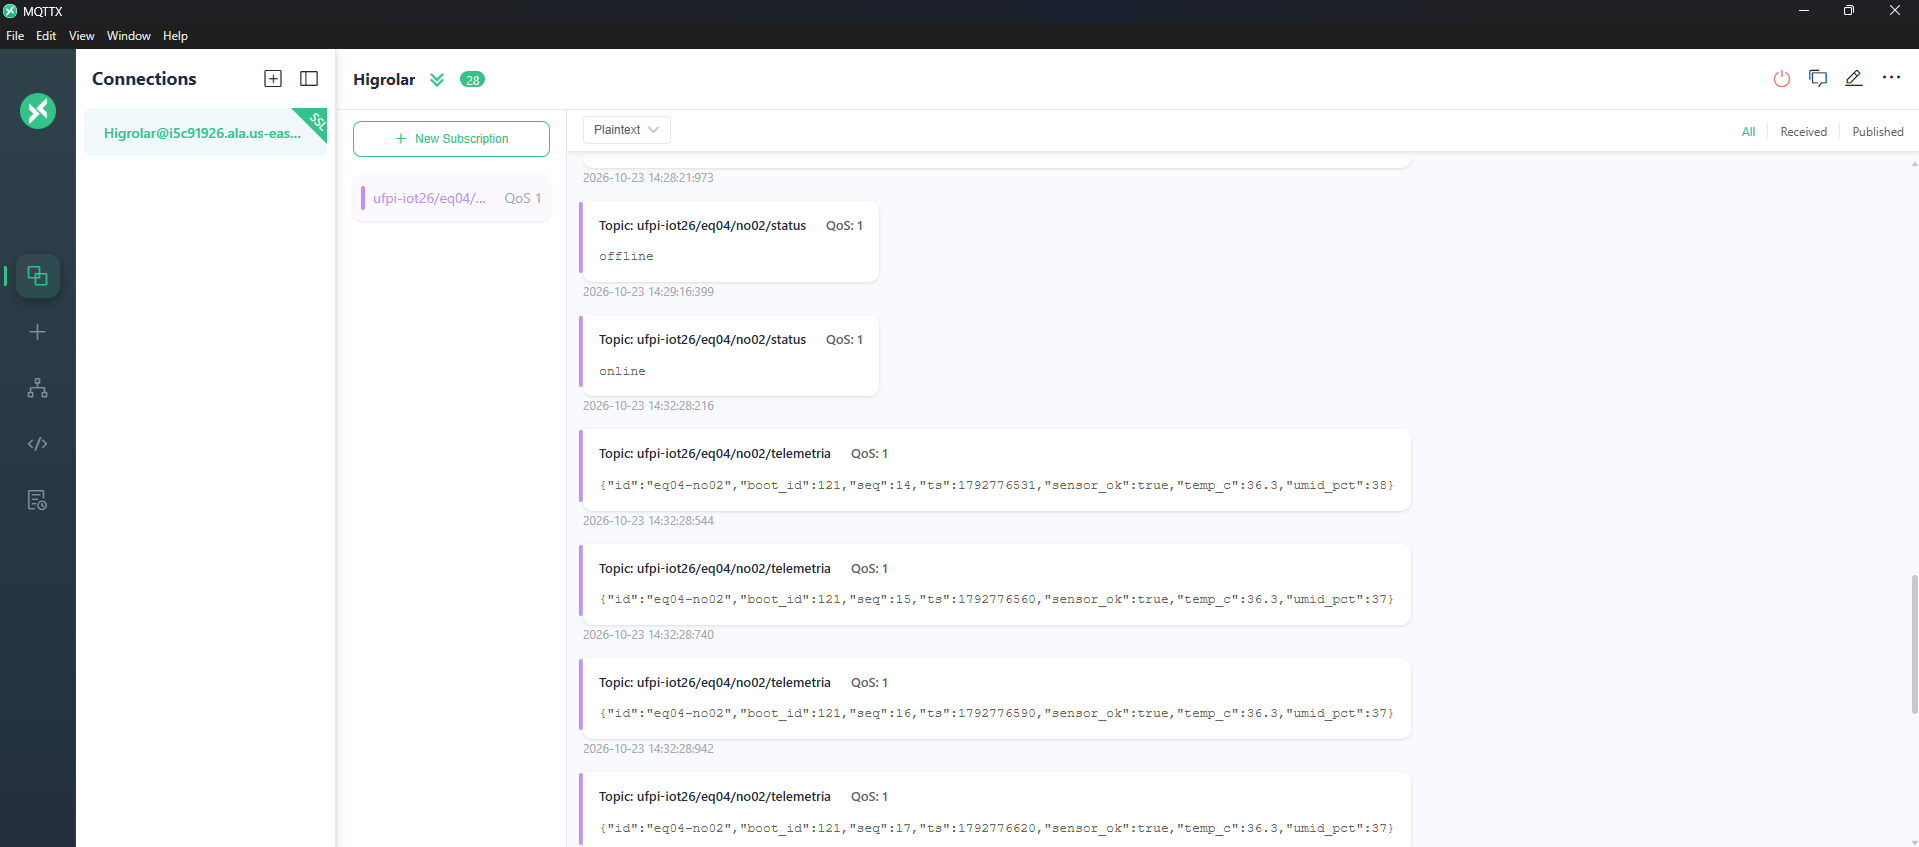
\includegraphics[width=.96\textwidth]{evidencias/prints/mqttx_wifi_retorno.png}\caption{MQTTX evidencia \texttt{offline}, \texttt{online} e retomada da telemetria.}\fonte{Evidência coletada pela equipe em 23/10.}\end{figure}
\begin{figure}[H]\centering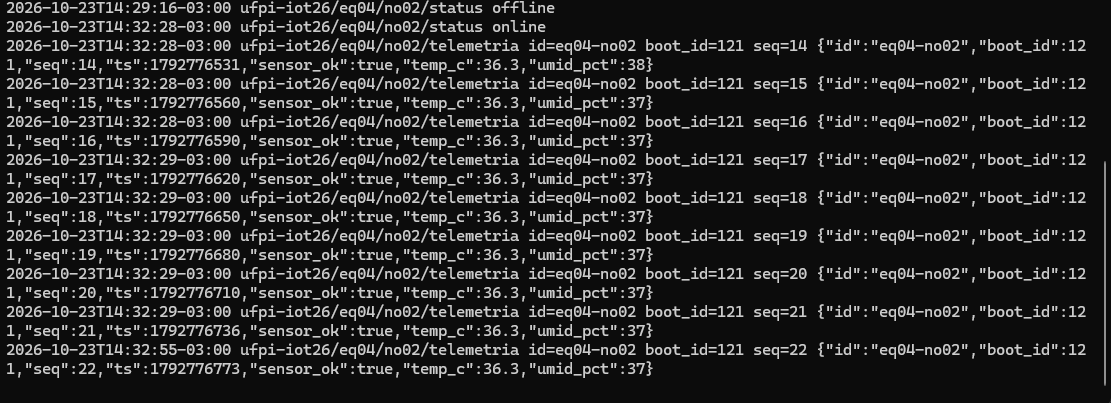
\includegraphics[width=.96\textwidth]{evidencias/prints/gravador_backlog.png}\caption{Console do gravador na recuperação de mensagens acumuladas.}\fonte{PowerShell da coleta eq04.}\end{figure}
\section{Reinício do ESP32, LWT e NTP}
O botão EN foi pressionado às 14h35 de 23/10. O histórico registra \texttt{boot\_id} 121 e depois 122; a sequência recomeça em 1 no novo boot. A primeira mensagem no boot 122 chegou com \texttt{ts:null}; a segunda passou a trazer tempo Unix. Houve eventos de \texttt{offline/online} registrados pelo broker, mas não se cronometrou o intervalo exato entre corte de energia e publicação do testamento. Um estado retido recebido quando o gravador se conecta não deve ser confundido com LWT disparado naquele mesmo instante.
\begin{figure}[H]\centering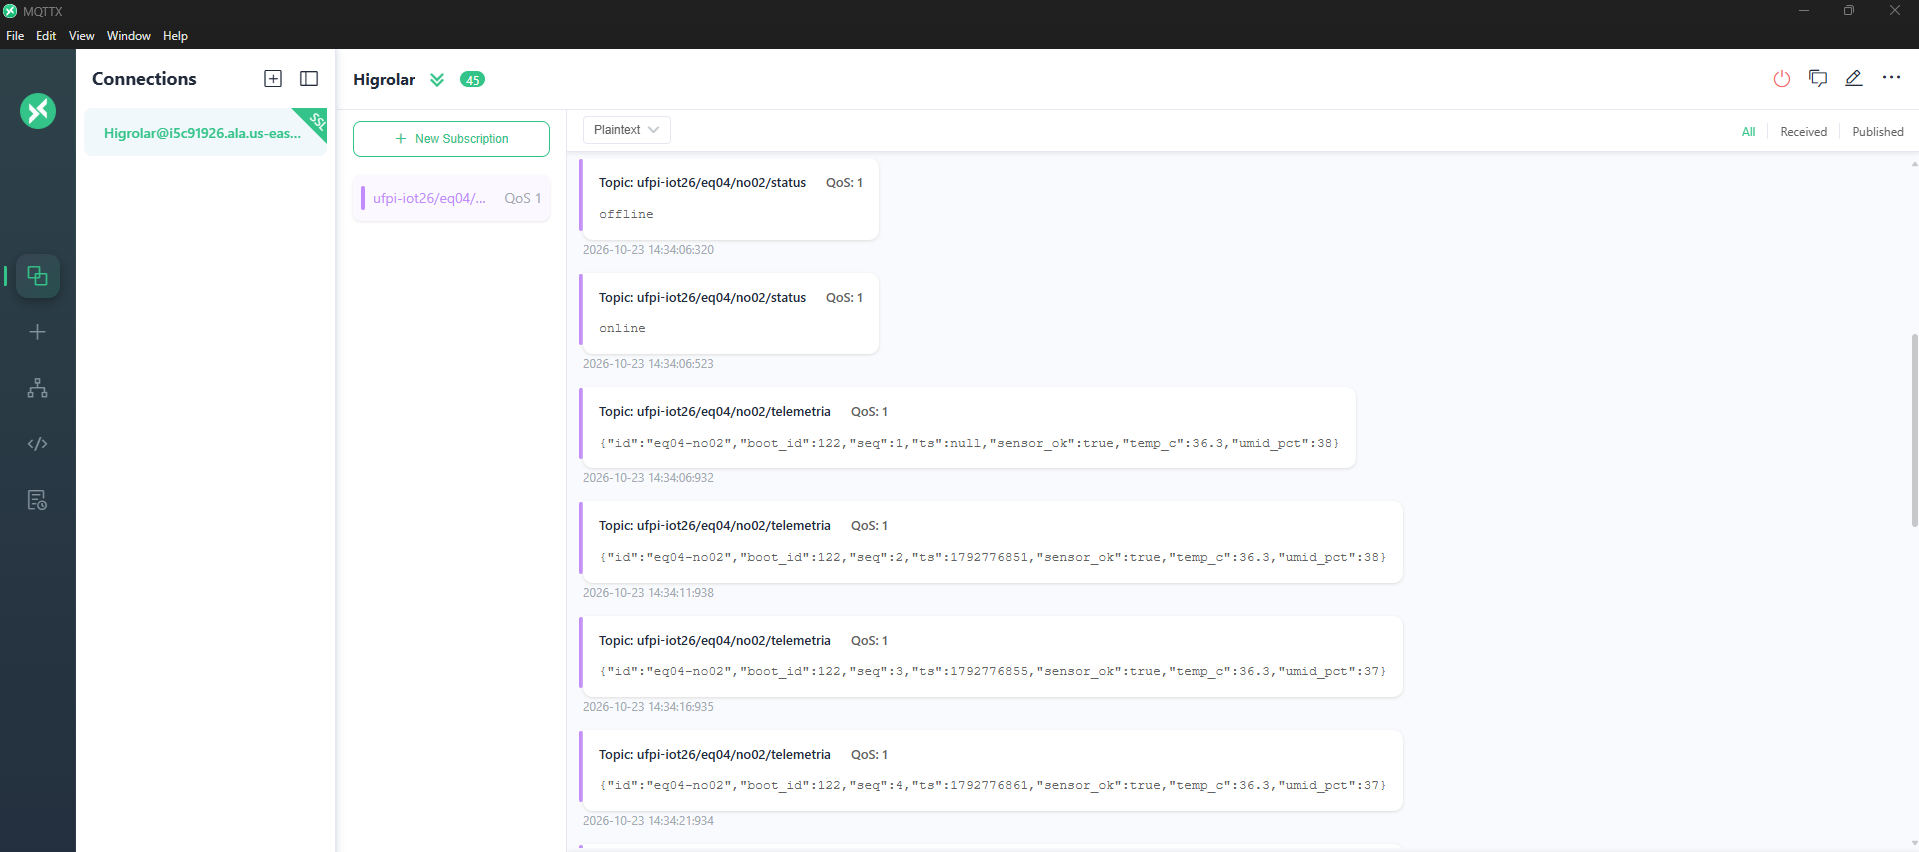
\includegraphics[width=.96\textwidth]{evidencias/prints/mqttx_ntp.png}\caption{Novo \texttt{boot\_id}, sequência reiniciada e primeira leitura antes do sincronismo NTP.}\fonte{MQTTX, 23/10 às 14h34.}\end{figure}
\section{Persistência do gravador e qualidade}
Às 14h38 foi reiniciado o processo de gravação. A conexão subsequente informou sessão anterior existente, com entregas em lote, retomando o CSV com novos registros. O \texttt{qualidade.py} conta duas duplicações lógicas no arquivo final, cuja chave é \texttt{(id,boot\_id,seq)}, mesmo com \texttt{DUP=0}; essa distinção é esperada em QoS 1 e comprova a necessidade de deduplicação \emph{depois} da captura do dado bruto. Um evento extra de \texttt{offline/online} ocorreu em 24/10 às 11h47, mas sua causa não foi identificada no diário; não se atribui artificialmente esse episódio a teste de rede.
\begin{figure}[H]\centering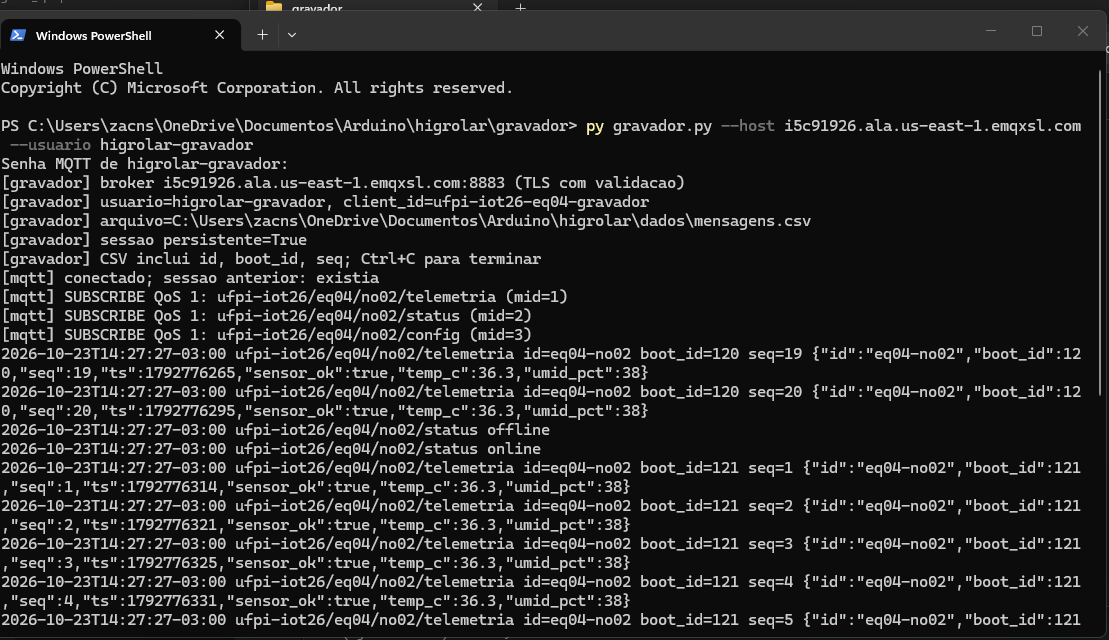
\includegraphics[width=.94\textwidth]{evidencias/prints/gravador_conexao.png}\caption{Inicialização do assinante com TLS, Client ID fixo, inscrição QoS 1 e recebimento de mensagens.}\fonte{PowerShell da equipe.}\end{figure}
\section{Resultados negativos, testes incompletos e reprodução}
O equipamento não dispõe de medição de corrente de Wi-Fi, nem foi aferido o intervalo entre o instante físico da queda de alimentação e a publicação do LWT. O TLS do nó usa \texttt{setInsecure()} quando não há CA embarcada; no EMQX o mecanismo de autorização está em blacklist, com comportamento permissivo fora das regras explícitas. Esses fatos reduzem a avaliação de segurança, mas são declarados para permitir reprodução honesta. O hardware não contém relé para controlar os aparelhos ambientais: as intervenções foram manuais e registradas no diário. A saída integral do programa de qualidade está no Apêndice F e o código correspondente em \texttt{gravador/}.

\chapter{Resultados e discussão}\label{cap:resultados}
\rubricaComunicacao
\section{Séries temporais finais da campanha}
A campanha final abrange 25h29min27s de dados de chegada; no subconjunto de 3.080 telemetrias logicamente únicas, a temperatura variou de 26,9 a 36,9~\si{\celsius}, e a umidade relativa de 34\% a 73\%. As Figuras~\ref{fig:temp-final} e~\ref{fig:ur-final} apresentam somente pontos medidos, sem interpolar temporalmente o período da queda de Wi-Fi. Os eventos de intervenção são marcados no eixo de tempo pelo diário; a escala representa hora local (UTC-3). Os gráficos não são certificados metrológicos do DHT11 e não demonstram generalização espacial do cômodo.
\begin{figure}[H]\centering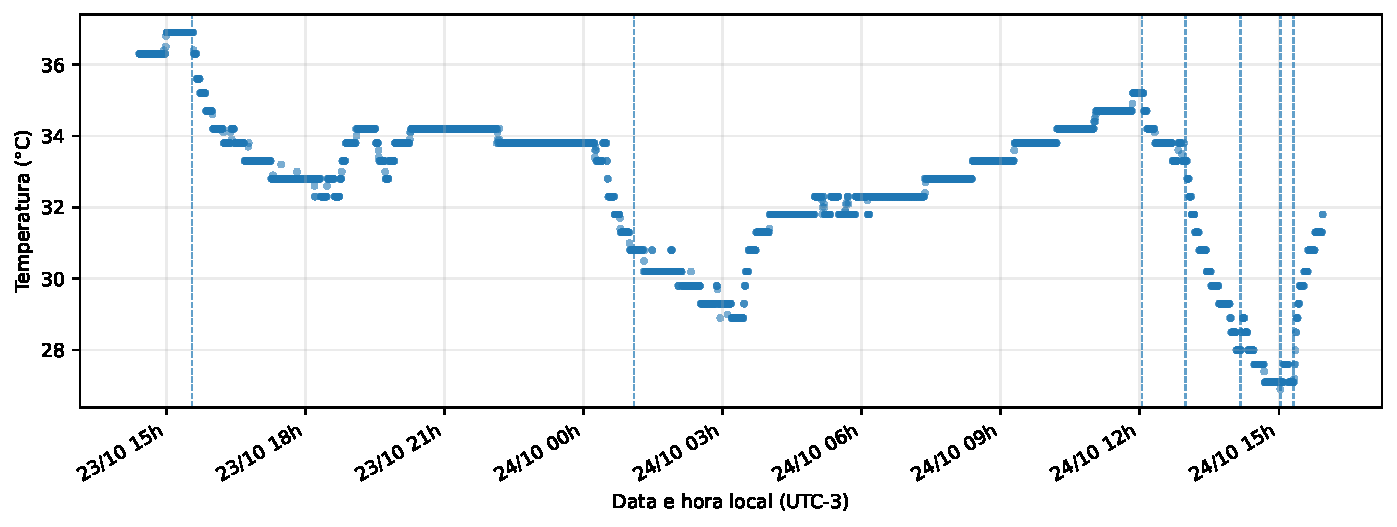
\includegraphics[width=\textwidth]{figuras/temperatura_serie_final.pdf}\caption{Série final de temperatura com intervenções indicadas por linhas verticais.}\label{fig:temp-final}\fonte{\texttt{dados/mensagens.csv}, telemetrias únicas, horário de aquisição válido ou recepção no único ponto com \texttt{ts:null}.}\end{figure}
\begin{figure}[H]\centering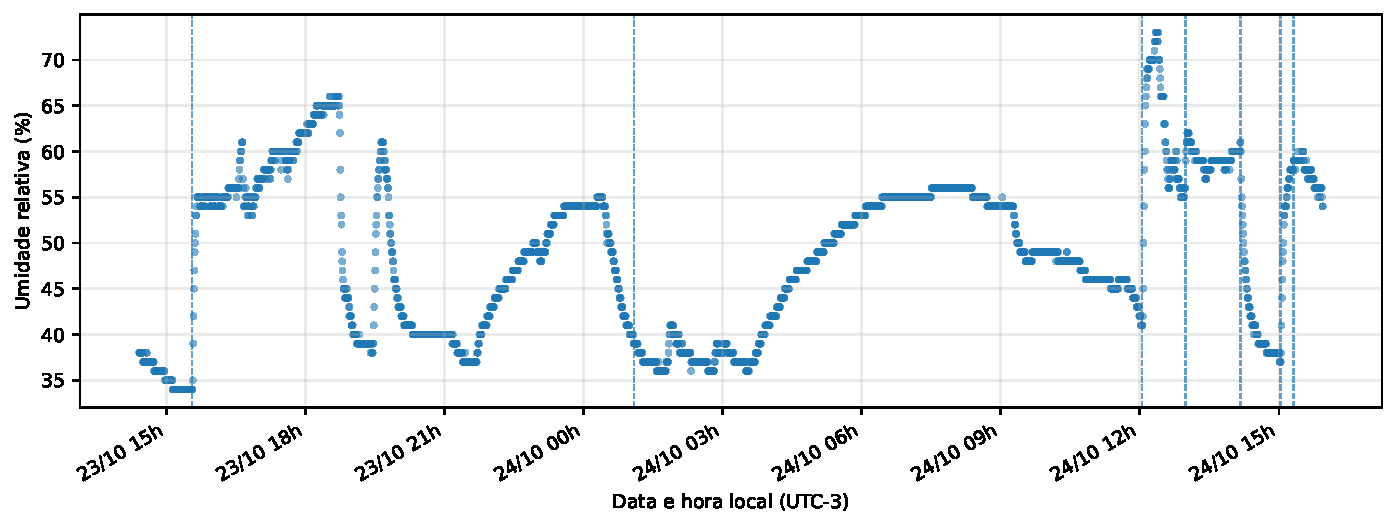
\includegraphics[width=\textwidth]{figuras/umidade_serie_final.pdf}\caption{Série final de umidade relativa, sem interpolação de lacunas.}\label{fig:ur-final}\fonte{CSV final e diário, 23--24/10/2026.}\end{figure}
\section{Umidificação isolada: primeira intervenção}
Em 23/10, às 15h33, o umidificador foi acionado manualmente. Duas janelas adjacentes de 30~min (15h03--15h33, antes; 15h33--16h03, após) contiveram 60 amostras válidas cada. A umidade média passou de 34,15\% para 52,87\% (diferença de +18,72 pontos percentuais), enquanto a temperatura média caiu de 36,90 para aproximadamente 35,22~\si{\celsius} (diferença de $-1,68$~\si{\celsius}). Esses contrastes são descritivos e associados temporalmente ao evento, sem grupo de controle, randomização nem estabilização do ambiente.
\begin{figure}[H]\centering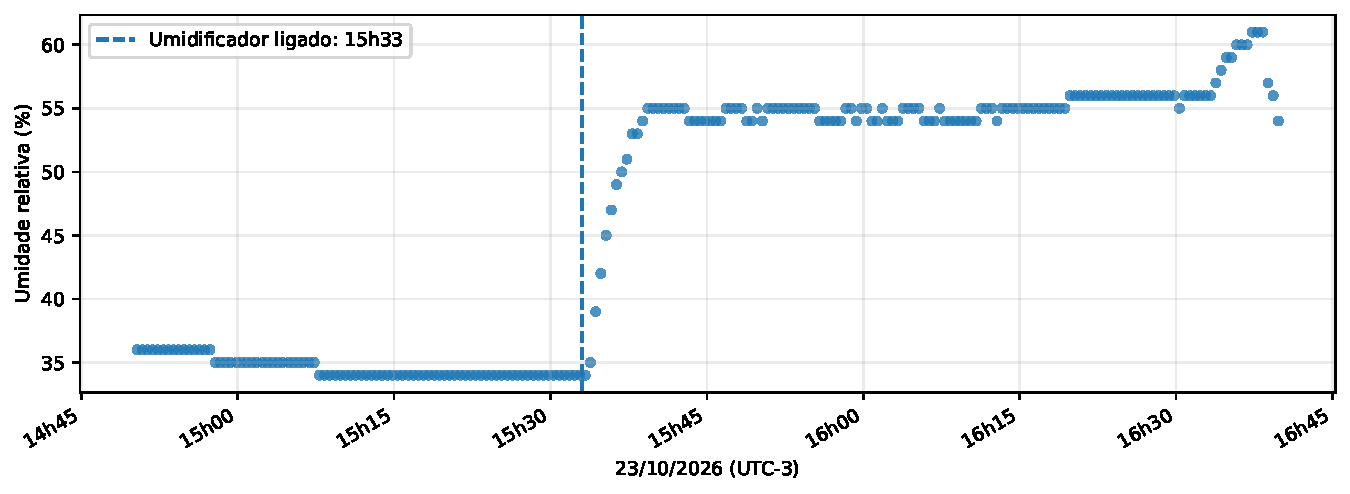
\includegraphics[width=.95\textwidth]{figuras/evento_umidificador_final.pdf}\caption{Umidade relativa na janela próxima ao acionamento de 23/10 às 15h33.}\fonte{CSV final, janelas explicitadas no texto.}\end{figure}
\begin{table}[H]\centering\caption{Comparação de 30 min antes e depois do primeiro acionamento}\label{tab:prepos}\footnotesize
\begin{tabular}{@{}L{6.3cm}R{2.45cm}R{2.45cm}R{2.7cm}@{}}\toprule
Variável&Antes ($n=60$)&Depois ($n=60$)&Diferença\\\midrule
Umidade relativa média (\%)&34,15&52,87&+18,72 p.p.\\
Temperatura média (\si{\celsius})&36,90&35,22&$-1,68$~\si{\celsius}\\\bottomrule\end{tabular}\fonte{Cálculo sobre CSV final; médias arredondadas.}\end{table}
A desativação às 18h43 foi seguida por variação no sentido oposto: a média de UR em 30~min antes era 64,97\%, contra 43,80\% nos 30~min posteriores; a temperatura média foi 32,56 versus 33,68~\si{\celsius}. Esses resultados são compatíveis com a dinâmica esperada, mas podem sofrer influência da circulação de ar e do posicionamento relativo do sensor.
\section{Refrigeração isolada durante a madrugada}
De 24/10 às 01h05 às 04h05, o diário registra ar-condicionado ajustado para 24~\si{\celsius}, com umidificador desligado. Durante as três horas, o dataset contém 360 telemetrias únicas, com médias observadas de 30,06~\si{\celsius} e 37,85\% UR. As médias medidas não devem ser confundidas com o ajuste de 24~\si{\celsius} do controle remoto: a temperatura junto ao DHT11 depende do cômodo, da distância, do tempo de resposta e das condições do ar. Na janela de 30~min posterior ao acionamento, a temperatura média foi 30,48~\si{\celsius} e a UR 37,50\%; imediatamente antes foram 31,48~\si{\celsius} e 43,52\%.
\section{Ensaio simultâneo de ar-condicionado e umidificador}\label{sec:experimento-combinado}
O diário permite distinguir duas fases de operação simultânea: \textbf{12h59--14h10} e \textbf{15h02--15h19}, ambas em 24/10. A primeira ocorre após ligar o umidificador às 12h03 e, 56 minutos depois, o ar-condicionado (ajustado para 24~\si{\celsius}). Na segunda, o umidificador é religado às 15h02 com o ar ainda ligado. Às 15h19, o ar é desligado \emph{e a janela é aberta}; portanto os 16 minutos seguintes não constituem condição de aparelho único em ambiente fechado. Às 15h35 o umidificador também é desligado. Todos os horários são do diário manual, não comandos acionados pelo nó IoT.
\begin{figure}[H]\centering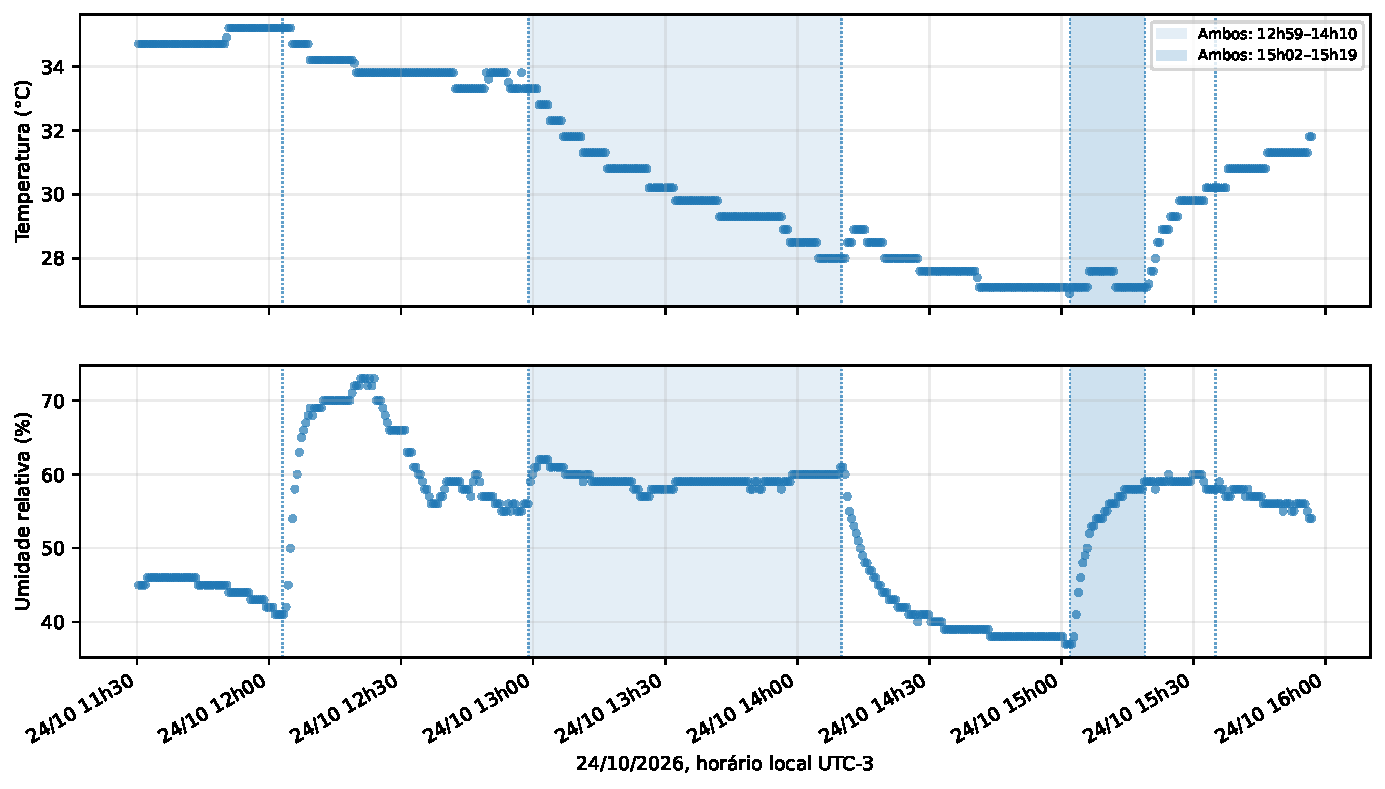
\includegraphics[width=\textwidth]{figuras/ensaio_simultaneo_final.pdf}\caption{Temperatura e umidade medidas na tarde de 24/10. Faixas sombreadas assinalam funcionamento simultâneo; linhas pontilhadas marcam intervenções registradas.}\label{fig:simultaneo}\fonte{3.080 telemetrias únicas do arquivo final e diário de eventos.}\end{figure}
\begin{table}[H]\centering\caption{Fases observadas em 24/10 e seus indicadores descritivos}\label{tab:fases}\scriptsize
\begin{tabular}{@{}L{5.5cm}C{1.25cm}C{2.15cm}C{2.15cm}L{3.2cm}@{}}\toprule
Condição / janela&$n$&Temperatura média&UR média&Observação\\\midrule
Umidificador, 12h03--12h59&112&33,89~\si{\celsius}&62,23\%&Antes do ar\\
Ambos ligados, 12h59--14h10&142&30,14~\si{\celsius}&59,28\%&Ar ajustado a 24~\si{\celsius}\\
Somente ar, 14h10--15h02&104&27,63~\si{\celsius}&41,34\%&Umidificador desligado\\
Ambos ligados, 15h02--15h19&34&27,28~\si{\celsius}&53,32\%&Segundo ensaio\\
Janela aberta e umidificador, 15h19--15h35&32&29,25~\si{\celsius}&59,00\%&Ar desligado; ventilação externa\\
Janela aberta, sem aparelhos, 15h35--15h56&44&30,99~\si{\celsius}&56,57\%&Fim da campanha\\\bottomrule\end{tabular}\fonte{Médias de telemetrias únicas cujos horários de aquisição estão nos intervalos semiabertos assinalados.}\end{table}
As janelas possuem extensões diferentes, e não houve controle de clima externo, potência real dos aparelhos nem distância exata ao sensor. Por isso, a diferença entre as médias das fases não representa efeito causal nem comparação experimental randomizada. Mesmo assim, a marcação temporal dos eventos torna o dataset adequado a rótulos exploratórios como \emph{umidificação isolada}, \emph{refrigeração isolada}, \emph{operação conjunta} e \emph{janela aberta}.
\section{Placar dos requisitos e passagem para a AP3}
Dos 13 requisitos da Tabela~\ref{tab:rastreabilidade}, 11 foram atendidos e 2 atendidos em parte; nenhum ficou sem atender. Os dois parciais são \RNF{05}, porque o nó não valida o certificado do servidor, e \RNF{06}, porque o custo do rádio não foi medido. As etapas de sensoriamento e gravação em CSV funcionaram: foram recebidas 3.082 telemetrias e o analisador identificou 3.080 únicas, com duas duplicações e sem saltos internos nos boots observados. O comando remoto alterou a periodicidade; sessões e reconexões foram demonstradas nos testes; os status retidos e o LWT apresentaram transições visíveis. Em contrapartida, a estimativa energética do rádio não foi aferida e o TLS embarcado não autenticou o certificado do servidor sem CA configurada. A autorização por \emph{blacklist} também é menos restritiva que uma política de negação por padrão. Para a AP3, o conjunto de dados oferece episódios anotados, mas requer coleta em outros dias e ambientes para formar base representativa e verificar generalização.

\chapter{Conclusões, limitações e próximos passos}\label{cap:conclusao}
\rubricaComunicacao
A segunda etapa do projeto Higrolar cumpriu o propósito de integrar o protótipo físico da AP1 à infraestrutura de comunicação e construir um dataset real e rastreável. A arquitetura baseada em ESP32, DHT11, OLED, Wi-Fi e EMQX Cloud ofereceu publicações MQTT com QoS 1, status retido, testamento \texttt{offline}, configuração remota do intervalo e um assinante Paho que persiste mensagens em disco. A segregação em três usuários MQTT documentou responsabilidades diferentes de dispositivo, monitor e gravador, embora o modo de ACL utilizado no EMQX tenha sido permissivo por padrão.
A campanha definitiva de 25h29min27s totalizou 3.096 mensagens, sendo 3.082 telemetrias e 3.080 telemetrias únicas, com duas duplicações lógicas, uma medição sem timestamp NTP e nenhum salto interno detectável entre sequências de um mesmo boot. A temperatura registrada variou de 26,9 a 36,9~\si{\celsius} e a umidade relativa entre 34\% e 73\%. O primeiro acionamento do umidificador coincidiu com aumento da média de UR de 34,15\% para 52,87\% em janelas adjacentes de 30~min. O ensaio posterior com ar-condicionado e umidificador simultâneos (12h59--14h10) registrou médias de 30,14~\si{\celsius} e 59,28\% de UR, enquanto um segundo trecho simultâneo ocorreu das 15h02 às 15h19. Essas observações não estabelecem causalidade porque os fatores ambientais não foram rigidamente controlados.
\section{Limitações observadas}
O DHT11 não é sensor metrológico de alta precisão e não é adequado para quantificar umidades extremamente baixas; o ponto físico não representa necessariamente todo o cômodo. A fila de 120 registros em RAM não resiste à falta de energia, embora o \texttt{boot\_id} sobreviva em NVS. O QoS 1 admite repetição, e 100\% de completude entre sequências numeradas não significa coleta perfeita entre todos os períodos operacionais. Durante a campanha, uma transição de estado em 24/10 às 11h47 não teve causa documentada. O atraso de chegada é influenciado por clocks e backlog. O custo real do rádio não foi medido; a autonomia permanece estimada com base na AP1, sem atualização instrumental da corrente de Wi-Fi. O gravador valida o certificado TLS no Windows, mas o firmware da campanha usa \texttt{setInsecure()} sem CA embarcada; a ACL do EMQX estava em modo blacklist.
\section{Perspectivas para o Módulo 3}
Como consequência prática, a equipe dispõe de um fluxo funcional do sensor ao CSV, de registros de estado e de eventos do mundo real com horário. No ciclo seguinte poderão ser criados rótulos exploratórios de intervenção, testadas regras de limiares e calculadas características temporais, preservando a diferença entre medição, evento relatado e inferência. Recomendam-se campanhas repetidas em dias distintos, identificação da posição do nó e dos equipamentos, endurecimento da ACL para negação por padrão, configuração de CA no ESP32 e medição direta de consumo elétrico. O firmware, gravador, analisador, diário, CSV bruto e fontes LaTeX integram o pacote entregue para reprodutibilidade.
\section{Divisão do trabalho}
Os papéis do \moduloDoCiclo\ rotacionaram em relação à AP1: ninguém repetiu o papel do ciclo anterior.
\begin{description}[style=unboxed, leftmargin=0.6cm]
  \item[Raimundo Nonato da Silva Sá Sobrinho (\emph{firmware} e comunicação; na AP1, integração).] Firmware de comunicação: conexão Wi-Fi e MQTT, reconexão, fila local, NTP e testamento.
  \item[Francisco de Assis Machado dos Santos (\emph{firmware} e comunicação; na AP1, documentação).] Contrato de dados e de tópicos, configuração remota do período e contas do EMQX.
  \item[Lemuel Cavalcante Lopes (integração; na AP1, \emph{firmware}).] Caminho do dado do sensor ao CSV, matriz de decisão de conectividade e rastreabilidade da Seção~\ref{sec:rastreabilidade}.
  \item[Zacarias do Nascimento Seriano Junnior (dados; na AP1, \emph{hardware}).] Gravador, condução da campanha de coleta, diário e registro de eventos, e execução do \texttt{qualidade.py}.
  \item[Thales Rodrigues Martins (documentação; na AP1, integração).] Redação e revisão deste relatório, descrição do conjunto de dados e declaração do Apêndice~\ref{ap:ia}.
\end{description}
\bigskip
\imprimirTabelaIntegrantes


% ---------- ELEMENTOS PÓS-TEXTUAIS -----------------------------------
\postextual

\chapter*{Referências}\addcontentsline{toc}{chapter}{Referências}
\noindent AL-FUQAHA, Ala et al. Internet of Things: a survey on enabling technologies, protocols, and applications. \textit{IEEE Communications Surveys \& Tutorials}, v. 17, n. 4, p. 2347--2376, 2015.\par\medskip
\noindent EQUIPE ESTIAGEM. \textit{Higrolar: monitor local de temperatura e umidade relativa do ar}. Relatório técnico da AP1. Universidade Federal do Piauí, 2026.\par\medskip
\noindent ESPRESSIF SYSTEMS. \textit{ESP32 series datasheet}. Versão 4.3. 2023.\par\medskip
\noindent UNIVERSIDADE FEDERAL DO PIAUÍ. \textit{Instruções de entrega do projeto da AP2: Tópicos em Sistemas Computacionais I}. Teresina: UFPI, 2026.\par\medskip
\noindent UNIVERSIDADE FEDERAL DO PIAUÍ. \textit{Laboratório 03: Telemetria dos sensores do projeto via MQTT}. Teresina: UFPI, 30 set. 2026.\par

\begin{apendicesenv}
  \partapendices
  \chapter{Mapa de barramento e interligações}\label{ap:barramento}
\begin{table}[H]\centering\caption{Mapa físico do Higrolar em campanha}\label{tab:barramento}\footnotesize
\begin{tabular}{@{}L{3cm}L{2.8cm}L{2.6cm}L{5.5cm}@{}}\toprule
\textbf{Componente}&\textbf{Pinos no ESP32}&\textbf{Interface}&\textbf{Observação}\\\midrule
DHT11&GPIO4, 3V3, GND&Digital proprietária&Leitura a cada 2 s; dados ambientais\\
OLED SSD1306&SDA=GPIO21, SCL=GPIO22&I\textsuperscript{2}C, endereço 0x3C&Display 128$\times$64; atualiza após mudança visual\\
ESP32 DevKit&USB&Alimentação / série&Programa grava via USB, rádio Wi-Fi embarcado\\
Roteador&Wi-Fi 2,4~GHz&802.11&Sem ligação física com nó\\
\bottomrule\end{tabular}\fonte{Esquema funcional utilizado pela equipe.}\end{table}
A alimentação dos módulos é de 3,3~V, com referência de terra comum, e não por sinais 5~V nos GPIOs. O OLED responde a \texttt{0x3C}; a interface de programação e depuração é o Monitor Serial a 115.200~Bd. A AP2 não acrescentou relé, motor nem sensor secundário ao circuito da AP1.

  \chapter{Orçamento de energia}\label{ap:energia}
\section{Base histórica da AP1 e limite da AP2}
A AP1 apresentou orçamento elétrico calculado por valores estimados de componentes: ESP32 sem rádio na faixa de 40 a 70~mA (valor central 55), OLED entre 10 e 25~mA (valor central 17,5), DHT11 até 1~mA. Seu cenário de operação com display permanentemente ativo resultou em corrente média estimada de 75,4~mA e consumo de 1.809~mA\,h/dia a 5~V. Esse resultado \textbf{não contempla adequadamente a variação de consumo do Wi-Fi e a negociação TLS da AP2}.
\begin{table}[H]\centering\caption{Valores de partida da AP1, todos estimados}\label{tab:energia}\footnotesize
\begin{tabular}{@{}L{5cm}R{2.8cm}L{5.7cm}@{}}\toprule
\textbf{Componente}&\textbf{Valor usado}&\textbf{Procedência}\\\midrule
ESP32 ativo, sem Wi-Fi&55~mA&Faixa de especificação adotada pela AP1\\
OLED ativo&17,5~mA&Estimativa da AP1\\
DHT11&1~mA&Estimativa conservadora da AP1\\
Conjunto (estados da AP1)&75,4~mA&Modelo de estados da AP1; sem medidor USB\\
\bottomrule\end{tabular}\fonte{Relatório entregue na AP1 da equipe Estiagem.}\end{table}
\section{Capacidade energética e análise de sensibilidade}
Para uma bateria nominal de 10.000~mA\,h especificada em células de 3,7~V e eficiência de 85\%, a energia útil estimada na USB é \(10\,\mathrm{Ah}\times3{,}7\,\mathrm{V}\times0{,}85=31{,}45\,\mathrm{Wh}\). A autonomia aproximada para uma corrente média \(I\) na USB de 5~V é \(t=31{,}45/(5I)\), com \(I\) em ampères. Os resultados são \emph{cenários} e não medições da campanha.
\begin{table}[H]\centering\caption{Autonomia potencial com a corrente média real (não medida)}\label{tab:sensibilidade}\footnotesize
\begin{tabular}{@{}R{2.5cm}R{2.5cm}R{2.8cm}L{5.9cm}@{}}\toprule
\textbf{Corrente}&\textbf{Potência}&\textbf{Autonomia}&\textbf{Interpretação}\\\midrule
50 mA&0,25 W&125,8 h&Hipótese otimista\\
75 mA&0,375 W&83,9 h&Referência da AP1, sem rádio quantificado\\
100 mA&0,50 W&62,9 h&Consumo maior, autonomia inferior\\
150 mA&0,75 W&41,9 h&Hipótese pessimista\\\bottomrule\end{tabular}\fonte{Cálculo sobre 31,45~Wh úteis; hipótese de eficiência.}\end{table}
\section{Ponto ainda não verificado}
A equipe não registrou um log com \texttt{millis()} medindo separadamente associação Wi-Fi/DHCP, sessão TLS e publish, nem leitura real de corrente com medidor USB em série. Logo, a rubrica de medição do rádio permanece \textbf{pendente}. Uma medição futura deverá amostrar corrente de repouso, Wi-Fi associado e transmissão, medir tempo de cada estado e estimar o consumo diário ponderado pelo período de 30~s. Não extrapolar a autonomia da AP1 como resultado medido da AP2.

  \chapter{Procedimentos de testes reproduzíveis}\label{ap:testes}
\begin{table}[H]\centering\caption{Guia de reprodução dos principais testes de resiliência}\label{tab:passo-testes}\scriptsize
\begin{tabular}{@{}L{2.1cm}L{5.2cm}L{6.5cm}@{}}\toprule
\textbf{Teste}&\textbf{Preparação e ação}&\textbf{Evidência / aceitação}\\\midrule
CT-01/02&Com rede ativa, assinar \texttt{ufpi-iot26/eq04/no02/\#} no MQTTX; enviar \texttt{\{"periodo\_s":30\}} ao tópico config&Observar dois timestamps de telemetria separados por cerca de 30~s, QoS~1\\
CT-03&Deixar nó em funcionamento, gravador no notebook e suspender apenas Wi-Fi do nó&Capturar \texttt{offline}, \texttt{online} e sequências recuperadas\\
CT-04&Interromper alimentação do nó durante a sessão MQTT&Confirmar LWT \texttt{offline}; não confundir com publicação voluntária\\
CT-05&Pressionar EN, aguardar nova telemetria&Verificar \texttt{boot\_id} incrementado; \texttt{seq} reiniciado\\
CT-06&Parar gravador, manter broker/nó, abrir novamente com mesmo client ID&Verificar mensagens pendentes e CSV sem truncamento\\
CT-07&Reiniciar nó e acompanhar os primeiros pacotes antes de NTP&Observar \texttt{ts:null} ou registrar quando o relógio sincroniza cedo demais para observação\\
CT-08&Executar \texttt{qualidade.py} contra cópia congelada do CSV&Comparar chaves compostas, duplicatas, lacunas internas e horários\\
\bottomrule\end{tabular}\fonte{Procedimentos da equipe adaptados do Laboratório 03.}\end{table}
Todos os testes que interrompem energia ou rede são feitos deliberadamente, com equipamento alimentado por fonte USB adequada, sem conectar/desconectar fios do circuito energizado. Manter registro de data e hora do evento no Apêndice~\ref{ap:campanha}.

  \chapter{Declaração de uso de inteligência artificial generativa}\label{ap:ia}
A equipe declara o uso de IA generativa como ferramenta auxiliar na redação desta versão do relatório, revisão de código e planejamento de análises, mantendo o dever de auditar resultados antes da submissão. A ferramenta não foi fonte de leituras do sensor: os valores quantitativos apresentados derivam dos registros CSV da equipe e foram reprocessados por scripts.
\begin{table}[H]\centering\caption{Transparência de utilização de IA na AP2}\label{tab:ia}\footnotesize
\begin{tabular}{@{}L{3.2cm}L{2.7cm}L{4.6cm}L{4.3cm}@{}}\toprule
\textbf{Etapa}&\textbf{Ferramenta}&\textbf{Atividade}&\textbf{Verificação exigida da equipe}\\\midrule
Firmware/integração&ChatGPT&Discussão de MQTT, reinício e identificação de mensagens&Compilação, observação no ESP32 e MQTTX\\
Gravador/analisador&ChatGPT&Revisão e adaptação dos scripts ao EMQX/TLS&Execução local sobre mensagens reais, conferência do CSV\\
Relatório e gráficos&ChatGPT&Organização de capítulos e geração preliminar dos textos/figuras&Releitura por todos, validação dos valores e citações\\
Revisão do relatório&Claude (Anthropic)&Conferência do relatório contra as instruções da AP2, \emph{script} \texttt{limpar.py} e tabelas do Capítulo~\ref{cap:conectividade} calculadas do CSV&Números reconferidos contra \texttt{mensagens.csv} e a saída do \texttt{qualidade.py}\\
Coleta e eventos&Sem IA no sensor&Leituras e ações humanas efetivamente observadas&Logs, CSV e diário de campo\\
\bottomrule\end{tabular}\fonte{Elaborada pela equipe.}\end{table}
\noindent\textbf{Declaração.} A equipe declara que o conteúdo deste relatório e do código a ele associado foi revisado e é compreendido por todos os integrantes, e que todo uso de ferramentas de inteligência artificial generativa está registrado na tabela acima.
\vspace{0.6cm}
\imprimirTabelaIntegrantes
\vspace{0.6cm}
\noindent\localEntrega, \dataEntrega.

  % Apêndices que só existem a partir da AP2 (campanha de coleta)
  \ifnum\value{ciclo}>1\relax
    \chapter{Checklist de prontidão para a campanha}\label{ap:checklist}
\begin{table}[H]\centering\caption{Prontidão para comunicação e aquisição, avaliada após a coleta}\label{tab:checklist}\scriptsize
\begin{tabular}{@{}C{.55cm}L{4.65cm}L{4.4cm}L{1.5cm}L{2.7cm}@{}}\toprule
\#&Critério&Evidência observável&Condição&Observação\\\midrule
1&Leitura sem laço de espera longo&Firmware e OLED&Sim&Tarefa 2~s\\
2&Keepalive MQTT configurado&\texttt{setKeepAlive(30)}&Sim&LWT\\
3&Status retido e testamento&12 mensagens de estado&Sim&Retido e transitório\\
4&Reconexão após perda de Wi-Fi&14h29--14h32&Sim&Backlog\\
5&Contrato e timestamp&JSON com \texttt{boot\_id}, \texttt{seq}, \texttt{ts}&Sim&Um \texttt{ts:null}\\
6&Reboot identificável&Boots 120, 121, 122&Sim&NVS\\
7&Fila local e descarte&120 entradas no código&Sim&Volátil\\
8&Gravador com sessão durável&Log \texttt{session\_present}&Sim&Reconexão\\
9&Gravação antes do ACK&\texttt{fsync+manual\_ack}&Sim&CSV\\
10&Análise da qualidade&\texttt{qualidade.py} final&Sim&3.096 mensagens\\
11&Segredos não versionados&\texttt{.gitignore} e example&Revisar&Conferir Git\\
12&Validação de TLS ponta a ponta&Python verifica; ESP32 não&Parcial&Configurar CA\\
13&Autorização por menor privilégio&Regras explícitas, modo blacklist&Parcial&Usar whitelist\\
14&Medição real do custo do rádio&Sem instrumento&Não&Limitação\\\bottomrule\end{tabular}\fonte{Código, EMQX, evidências e campanha do Higrolar.}\end{table}
\section*{Síntese de prontidão}
A cadeia funcional de telemetria, persistência e qualidade foi concluída e testada com dados reais. A prontidão de segurança ainda depende da validação de certificado no nó e da configuração do EMQX para negar o acesso que não corresponda a uma regra explícita. O consumo do rádio tampouco foi medido. Essas limitações são parte do resultado da AP2, não itens marcados como concluídos sem evidência.

    \chapter{Registro da campanha de coleta}\label{ap:campanha}
\section*{Diário de testes operacionais}
O diário a seguir combina intervenções registradas manualmente e instantes de mensagens encontrados no CSV. Uma ocorrência \texttt{offline/online} sem anotação de intervenção é preservada como causa desconhecida, sem interpretação especulativa.
\begin{table}[H]\centering\caption{Eventos operacionais e mensagens de estado, UTC-3}\label{tab:diario}\scriptsize
\begin{tabular}{@{}L{3.15cm}L{6.55cm}L{4.5cm}@{}}\toprule
Data e hora&Evento documentado&Procedência\\\midrule
23/10 14h27&Gravador conectado com sessão MQTT existente&PowerShell e CSV\\
23/10 14h29&Interrupção proposital do Wi-Fi do ESP32&Diário original\\
23/10 14h29min16s&\texttt{offline} observado no broker&CSV de status\\
23/10 14h32min28s&\texttt{online}, telemetrias com backlog&CSV e gravador\\
23/10 14h35&Reinício por botão EN&Diário; novo boot 122\\
23/10 14h38&Encerramento e reinício do processo \texttt{gravador.py}&Diário e logs Python\\
23/10 14h42min22s&\texttt{offline} transitório&CSV, causa não aferida\\
23/10 14h42min24s&\texttt{online}, repetição lógica identificada&CSV, chave composta\\
24/10 11h47min25s&\texttt{offline} não provocado/documentado&CSV de status\\
24/10 11h47min26s&\texttt{online} recuperado&CSV de status\\
24/10 15h56min54s&Última mensagem do arquivo final&CSV consolidado\\\bottomrule\end{tabular}\fonte{\texttt{dados/mensagens.csv}, logs e diário de eventos.}\end{table}
\section*{Diário ambiental para rotulagem posterior}
\begin{table}[H]\centering\caption{Eventos manuais da campanha, com começo e fim quando anotados}\label{tab:eventos}\scriptsize
\begin{tabular}{@{}L{3.2cm}L{3.1cm}L{5.8cm}L{2.4cm}@{}}\toprule
Início&Fim&Condição ambiental observada&Registro\\\midrule
23/10 15h33&23/10 18h43&Umidificador ligado, ar não registrado&Diário\\
24/10 01h05&24/10 04h05&Ar-condicionado ligado; ajuste 24~\si{\celsius}&Diário\\
24/10 12h03&24/10 12h59&Umidificador ligado, antes de ligar o ar&Diário\\
24/10 12h59&24/10 14h10&Umidificador e ar ligados simultaneamente&Diário\\
24/10 14h10&24/10 15h02&Ar ligado, umidificador desligado&Diário\\
24/10 15h02&24/10 15h19&Ar e umidificador ligados simultaneamente&Diário\\
24/10 15h19&24/10 15h35&Ar desligado; janela aberta; umidificador ligado&Diário\\
24/10 15h35&24/10 15h56&Umidificador desligado, janela aberta anteriormente&Diário\\\bottomrule\end{tabular}\fonte{\texttt{5 - Log Eventos Relatório(2).txt}; horas locais UTC-3.}\end{table}
\section*{Saída integral do analisador sobre o arquivo definitivo}
A listagem é a saída integral do analisador executado sobre o CSV final de 3.096 mensagens. As mesmas contagens fundamentam as Tabelas~\ref{tab:qualidade} e~\ref{tab:campanha}.
\lstinputlisting[style=terminal,basicstyle=\ttfamily\tiny,breaklines=true,caption={Relatório final de qualidade, emitido pelo analisador da equipe},label={lst:qualidade-final}]{evidencias/qualidade_final.txt}
\section*{Arquivos brutos e evidências complementares}
Os arquivos estão organizados nas pastas \texttt{docs/evidencias/}, \texttt{dados/} e \texttt{gravador/}. As figuras do corpo do relatório são geradas por \texttt{dados/gerar\_graficos.py}. A saída CSV original não foi sobrescrita por dados deduplicados ou interpolados.

  \fi
\end{apendicesenv}

\end{document}
